\documentclass[11pt,a4paper]{article}
\usepackage{lmodern}


\usepackage{amssymb,amsmath}
\usepackage{ifxetex,ifluatex}
\usepackage{fixltx2e} % provides \textsubscript
\ifnum 0\ifxetex 1\fi\ifluatex 1\fi=0 % if pdftex
  \usepackage[T1]{fontenc}
  \usepackage[utf8]{inputenc}
\else % if luatex or xelatex
  \ifxetex
    \usepackage{mathspec}
    \usepackage{xltxtra,xunicode}
  \else
    \usepackage{fontspec}
  \fi
  \defaultfontfeatures{Mapping=tex-text,Scale=MatchLowercase}
  \newcommand{\euro}{€}
\fi
% use upquote if available, for straight quotes in verbatim environments
\IfFileExists{upquote.sty}{\usepackage{upquote}}{}
% use microtype if available

\usepackage[lmargin=3cm,rmargin=2.5cm,tmargin=2.5cm,bmargin=2.5cm]{geometry}

% Figure Placement:
\usepackage{float}
\let\origfigure\figure
\let\endorigfigure\endfigure
\renewenvironment{figure}[1][2] {
    \expandafter\origfigure\expandafter[H]
} {
    \endorigfigure
}

%% citation setup

\usepackage{csquotes}

\usepackage[backend=biber, maxbibnames = 99, style = apa]{biblatex}
\setlength\bibitemsep{1.5\itemsep}
\bibliography{Resources/references.bib}
\usepackage{longtable,booktabs}
\usepackage{graphicx}
\makeatletter
\def\maxwidth{\ifdim\Gin@nat@width>\linewidth\linewidth\else\Gin@nat@width\fi}
\def\maxheight{\ifdim\Gin@nat@height>\textheight\textheight\else\Gin@nat@height\fi}
\makeatother
% Scale images if necessary, so that they will not overflow the page
% margins by default, and it is still possible to overwrite the defaults
% using explicit options in \includegraphics[width, height, ...]{}
\setkeys{Gin}{width=\maxwidth,height=\maxheight,keepaspectratio}
\ifxetex
  \usepackage[setpagesize=false, % page size defined by xetex
              unicode=false, % unicode breaks when used with xetex
              xetex]{hyperref}
\else
  \usepackage[unicode=true]{hyperref}
\fi
\hypersetup{breaklinks=true,
            bookmarks=true,
            pdfauthor={Rezaul Hoque, Sarah Al-Talal},
            pdftitle={Predicting Residential Construction Year and
Classifying Architectural Typology},
            colorlinks=true,
            citecolor=blue,
            urlcolor=blue,
            linkcolor=black,
            pdfborder={0 0 0}}
\urlstyle{same}  % don't use monospace font for urls
\setlength{\parindent}{0pt}
\setlength{\parskip}{6pt plus 2pt minus 1pt}
\setlength{\emergencystretch}{3em}  % prevent overfull lines
\setcounter{secnumdepth}{5}

%%% Use protect on footnotes to avoid problems with footnotes in titles
\let\rmarkdownfootnote\footnote%
\def\footnote{\protect\rmarkdownfootnote}

%%% Change title format to be more compact
\usepackage{titling}

% Acronyms package defining
\urlstyle{same}  % don't use monospace font for urls

% Create subtitle command for use in maketitle
\newcommand{\subtitle}[1]{
  \posttitle{
    \begin{center}\large#1\end{center}
    }
}

\setlength{\droptitle}{-2em}
  \title{Predicting Residential Construction Year and Classifying
Architectural Typology}
  \pretitle{\vspace{\droptitle}\centering\huge}
  \posttitle{\par}
  \author{Rezaul Hoque, Sarah Al-Talal}
  \preauthor{\centering\large\emph}
  \postauthor{\par}
  \predate{\centering\large\emph}
  \postdate{\par}
  \date{today}

\usepackage{array}
\usepackage{calc}
\providecommand{\real}[1]{#1}
\providecommand{\tightlist}{\setlength{\itemsep}{0pt}\setlength{\parskip}{0pt}}
\let\oldsection\section
\renewcommand{\section}{\clearpage\oldsection}

%% linespread settings

\usepackage{setspace}

\onehalfspacing

% Language Setup

\usepackage{ifthen}
\usepackage{iflang}
\usepackage[super]{nth}

\ifthenelse{\equal{english}{german}}{
  \usepackage[ngerman]{babel}
  }{
  \usepackage[english]{babel}
  }

\IfFileExists{microtype.sty}{%
	\usepackage[nopatch=footnote]{microtype}
	\UseMicrotypeSet[protrusion]{basicmath} % disable protrusion for tt fonts
}{}

% escape pandocbounded
\newcommand{\pandocbounded}[1]{#1}

\begin{document}

\newgeometry{left=2cm,right=1cm,bottom=2cm,top=2cm}

\begin{titlepage}
  \noindent\begin{minipage}{0.6\textwidth}
	  \IfLanguageName{english}{University of Duisburg-Essen}{Universität Duisburg-Essen}\\
	  \IfLanguageName{english}{Faculty of Business Administration and Economics}{Fakultät für Wirtschaftswissensschaften}\\
	  \IfLanguageName{english}{Chair of Econometrics}{Lehrstuhl für Ökonometrie}\\
  \end{minipage}
	\begin{minipage}{0.4\textwidth}
	  \begin{flushright}
  	  \vspace{-0.5cm}
      \IfLanguageName{english}{\includegraphics*[width=5cm]{Resources/duelogo_en.png}}{\includegraphics*[width=5cm]{Resources/duelogo_de.png}}
	  \end{flushright}
	\end{minipage}
  \\
  \vspace{1.5cm}
  \begin{center}
  \huge{Predicting Residential Construction Year and Classifying
Architectural Typology}\\
  \vspace{0.5cm}
  \large{Term Paper}\\
  \vspace{1cm}
  \large{
  \IfLanguageName{english}{Submitted to the Faculty of \\ Business Administration and Economics \\at the \\University of Duisburg-Essen}{Vorgelegt der \\Fakultät für Wirtschaftswissenschaften der \\ Universität Duisburg-Essen}\\}
  \vspace{0.75cm}
  \large{\IfLanguageName{english}{from:}{von:}}\\
  \vspace{0.5cm}
  Rezaul Hoque, Sarah Al-Talal\\
  \end{center}
  \vspace{4cm}



  \noindent\begin{minipage}[t]{0.5\textwidth}
  \IfLanguageName{english}{Matriculation Number:}{Matrikelnummer}
  \end{minipage}
  \begin{minipage}[t]{0.7\textwidth}
  \hspace{1cm}, 
  \end{minipage}

  \noindent\begin{minipage}[t]{0.5\textwidth}
  \IfLanguageName{english}{Study Path:}{Studienfach:}
  \end{minipage}
  \begin{minipage}[t]{0.7\textwidth}
  \hspace{1cm}Information Systems
  \end{minipage}

  \noindent\begin{minipage}[t]{0.5\textwidth}
  \IfLanguageName{english}{Reviewer:}{Erstgutachter:}
  \end{minipage}
  \begin{minipage}[t]{0.7\textwidth}
  \hspace{1cm}Prof.~Dr.~Thomas Deckers
  \end{minipage}

  \noindent\begin{minipage}[t]{0.5\textwidth}
  \IfLanguageName{english}{Secondary Reviewer:}{Zweitgutachter}
  \end{minipage}
  \begin{minipage}[t]{0.7\textwidth}
  \hspace{1cm}M. Sc. Saskia Schütte
  \end{minipage}

  \noindent\begin{minipage}[t]{0.5\textwidth}
  \IfLanguageName{english}{Semester:}{Semester:}
  \end{minipage}
  \begin{minipage}[t]{0.7\textwidth}
  \hspace{1cm}Summer Semester
  \end{minipage}


  \noindent\begin{minipage}[t]{0.5\textwidth}
  \IfLanguageName{english}{Deadline:}{Abgabefrist:}
  \end{minipage}
  \begin{minipage}[t]{0.7\textwidth}
  \hspace{1cm}Aug 28, 2026
  \end{minipage}

\end{titlepage}


% Ends the declared geometry for the titlepage
\restoregeometry


\pagenumbering{Roman}
{
\hypersetup{linkcolor=black}
\setcounter{tocdepth}{3}
\tableofcontents
}

\newpage
\listoftables
\newpage
\listoffigures
\newpage
\pagenumbering{arabic}

\section{Introduction}\label{introduction}

The Ames Housing Dataset \autocite{DeCock2011} records 2,930 residential
property sales in Ames, Iowa between 2006 and 2010, described across 82
variables spanning physical dimensions, material quality, basement and
garage attributes and neighbourhood classification. Most work on this
dataset points toward one target: sale price. This study points
somewhere else: toward the structural and architectural information
already sitting in each property's physical record.

A fair amount of that other work already exists: machine learning has
been applied to the Ames dataset and comparable sources to forecast sale
price directly and to work out which housing characteristics move the
market most \autocite{ChoyHo2023,HoTangWong2020,JinXu2025}.

Two prediction problems drive the analysis here, each built around its
own research question.

\textbf{RQ1 (Regression: Predicting the Age of a House):} How accurately
can a machine learning model predict a residential property's original
construction year based solely on its current structural materials,
layout configuration and quality ratings, with no temporal metadata and
no market data in sight? The working assumption is that construction era
leaves a trace: in material choices, room configurations and the
amenities that came and went across the twentieth century.

\textbf{RQ2 (Classification: Automated Architectural Typology
Inference):} Can machine learning algorithms accurately infer a
residential property's architectural typology from its measurable
spatial footprint, structural scale metrics and internal layout
configuration alone, and which physical attributes serve as the most
discriminative geometric boundaries between single-story, multi-story,
one-and-a-half story and split-level residential typologies within the
Ames, Iowa housing stock?

Section \ref{practical-implications} returns to why recovering either
quantity is useful in practice, once the two attributes that would
normally supply this information (a construction date and a style label)
cannot be assumed to already be on file.

The two tasks are kept independent, though they share a single
preprocessing pipeline. Nine regression algorithms and eight classifiers
are compared, chosen to span the range from interpretable linear models
to opaque ensembles. Predictive performance matters throughout, but so
does a question that gets asked less often: how much can each model
class actually tell us about why it made a given prediction? All
preprocessing, modelling and evaluation described below was implemented
in Python (scikit-learn, XGBoost, category-encoders); this R Markdown
document is used only to report and discuss those results.

\section{Exploratory Data Analysis}\label{exploratory-data-analysis}

The dataset used here contains 2,930 residential property observations
across 82 variables, two of which (\texttt{Order}, \texttt{PID}) are
administrative identifiers rather than real predictors. What remains
covers structural, spatial and qualitative characteristics for each
property sold in Ames, Iowa; there is enough variety, in fact, that the
dataset lends itself naturally to supervised learning.

Roughly half the variables are numerical (lot area, above-ground living
area, garage capacity, construction year, basement size), and the rest
are categorical: neighborhood, building type, exterior materials,
heating quality, roof style, kitchen quality. Mixing measurable
quantities with qualitative ratings gives the models something more
interesting to work with than either type alone would provide.

Two supervised learning tasks are built on top of it: regression
predicts construction year (\texttt{Year\ Built}), and classification
predicts architectural style (\texttt{House\ Style}). Everything else,
once it has passed through the preprocessing described in Chapter 3,
becomes a predictor.

Table 1 summarises the dataset before preprocessing begins.

\begin{longtable}[]{@{}ll@{}}
\caption{Dataset
Characteristics.}\label{tbl-dataset-characteristics}\tabularnewline
\toprule\noalign{}
Characteristics & Value \\
\midrule\noalign{}
\endfirsthead
\toprule\noalign{}
Characteristics & Value \\
\midrule\noalign{}
\endhead
\bottomrule\noalign{}
\endlastfoot
Dataset & Ames Housing Dataset \autocite{DeCock2011} \\
Observations & 2,930 \\
Variables & 82 \\
Numerical Variables & 39 \\
Categorical Variables & 43 \\
Regression Target & Year Built \\
Classification Target & House Style \\
\end{longtable}

\subsection{Target Variable
Distributions}\label{target-variable-distributions}

\textbf{Year Built.} Construction years in the sample run from 1872 to
2010, averaging 1971.4 with a standard deviation of 30.2 years. The
distribution leans left (skewness = \(-0.604\), kurtosis = \(-0.502\)):
only a handful of nineteenth-century properties made it into the sample,
while the bulk of the housing stock dates from the mid-twentieth century
onward, an accumulation pattern that says more about which houses
survived than anything else. Figure \ref{fig:yearbuilt} shows the shape.

\begin{figure}[htbp]

{\centering 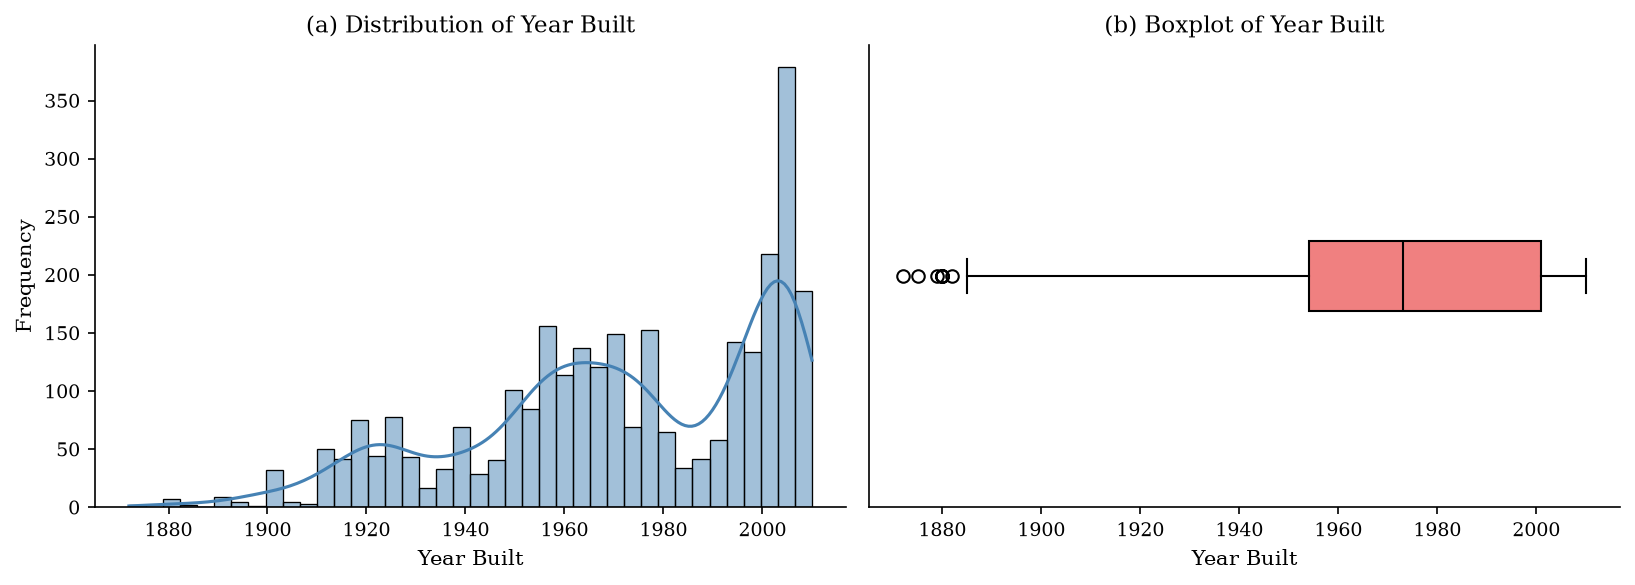
\includegraphics[width=\textwidth]{../figures/fig_yearbuilt_dist} 

}

\caption{\label{fig:yearbuilt}Distribution of Year Built: histogram with kernel density estimate (left) and boxplot (right). The left-skewed shape reflects the uneven historical accumulation of housing stock in the dataset.}\label{fig:fig-yearbuilt}
\end{figure}

\textbf{House Style.} The raw dataset records eight architectural style
codes, which are collapsed here into four typology classes: Single-story
(n = 1,481; 50.5\%), Multi-story (n = 905; 30.9\%), 1.5-story (n = 333;
11.4\%) and Split-level (n = 211; 7.2\%). The imbalance is hard to miss:
Single-story alone outnumbers the next largest class by more than two to
one, and it shapes which evaluation metric makes sense for
classification, a point picked up in Section \ref{model-selection}.
Figure \ref{fig:housestyle} shows the class counts before and after
consolidation.

\begin{figure}[htbp]

{\centering 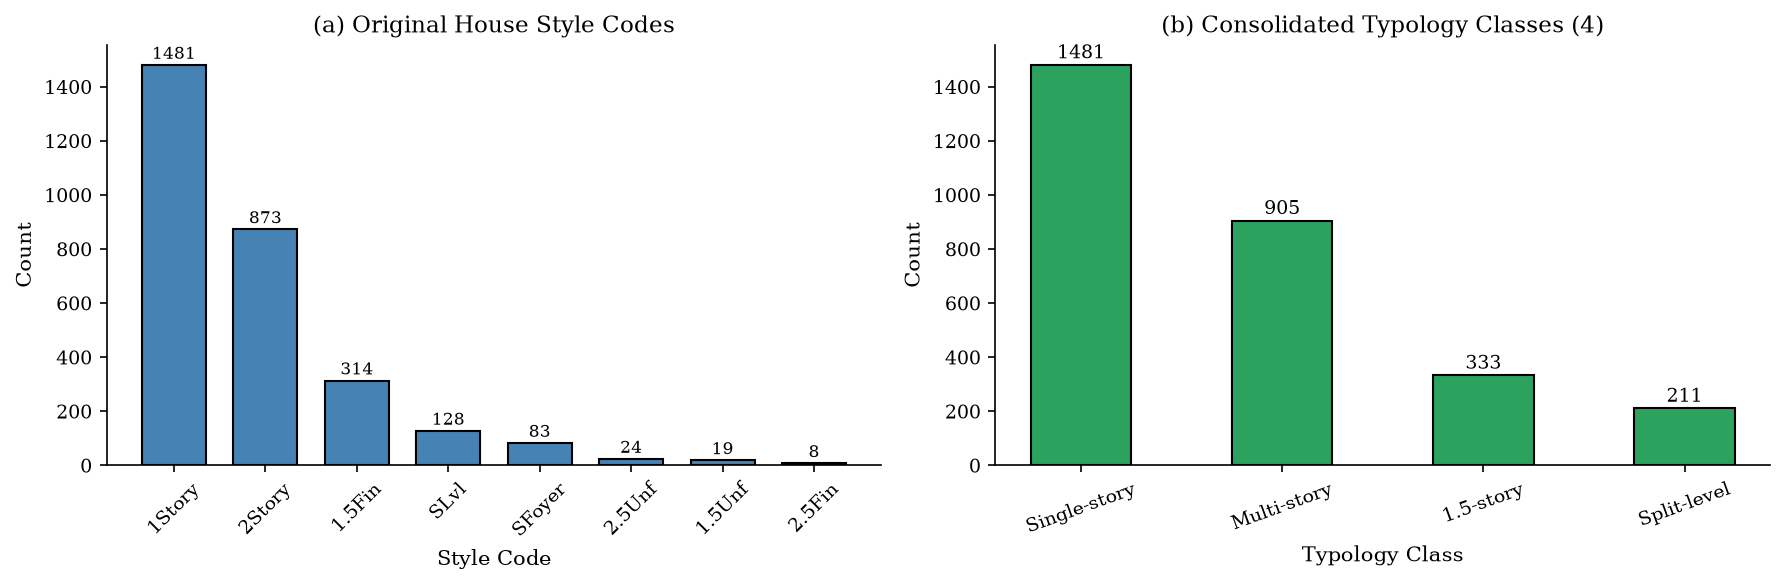
\includegraphics[width=\textwidth]{../figures/fig_housestyle_dist} 

}

\caption{\label{fig:housestyle}House Style distribution. Left: the original eight style codes. Right: the four typology classes used in modelling, formed by grouping related codes.}\label{fig:fig-housestyle}
\end{figure}

\subsection{Predictor Relationships}\label{predictor-relationships}

Pearson correlations between numerical predictors and Year Built (Figure
\ref{fig:correlation}, Appendix) identify Garage Year Built as the
strongest (\(r = 0.83\)), unsurprising since garages are usually built
alongside the house, followed by Overall Quality (\(r = 0.60\)),
tracking the shift toward higher-grade materials in newer construction.
Ground Living Area makes the top twelve by rank only (\(r = 0.24\)).
Older residential conventions show up on the negative side, in features
like Enclosed Porch area and Overall Condition.
\texttt{Garage\ Yr\ Blt}'s strong showing here is exactly why it is
excluded from the regression feature set (Section
\ref{encoding-and-scaling}): it is itself another construction-date
field, and keeping it as a predictor would run against RQ1's framing of
recovering construction year from physical attributes alone, with no
other temporal metadata in play.

\subsection{Classification Predictors}\label{classification-predictors}

The classification task uses a different, purely numeric feature set
(described in Chapter 3), so it is worth checking whether any of these
geometric predictors visibly separate the four typology classes before
any classifier is trained. Figure \ref{fig:clf-eda} shows three of them.
\texttt{2nd\ Flr\ SF} is the clearest separator: it sits at or near zero
for Single-story and Split-level properties, but is consistently
positive for Multi-story ones, with 1.5-story properties in between,
exactly what the class definitions would predict, since only Multi-story
and 1.5-story homes have a (partial or full) second floor by
construction. \texttt{Gr\ Liv\ Area} and \texttt{TotRms\ AbvGrd} both
increase from Split-level through Single-story and 1.5-story to
Multi-story, but with substantial overlap between classes, so neither is
a clean separator on its own. These are observed associations, not
evidence that floor area or room count \emph{causes} a particular
architectural form: a house's typology is fixed at construction and
simply co-occurs with these measurements.

\begin{figure}[htbp]

{\centering \includegraphics[width=\textwidth]{../figures/fig_clf_eda} 

}

\caption{\label{fig:clf-eda}Three classification predictors (`2nd Flr SF`, `Gr Liv Area`, `TotRms AbvGrd`) grouped by architectural typology class.}\label{fig:fig-clf-eda}
\end{figure}

\section{Data Preprocessing}\label{data-preprocessing}

\subsection{Missing Value Handling}\label{missing-value-handling}

Four columns were dropped before any modelling began: \texttt{Alley},
\texttt{Pool\ QC}, \texttt{Fence} and \texttt{Misc\ Feature}, all
missing more than 70\% of their values. Imputing at that level of
missingness would mean inventing most of a variable's distribution,
which defeats the purpose. That left 78 variables. Rows missing either
target variable were then removed as well, leaving all 2,930
observations usable.

Everything else with missing values gets imputed inside the modelling
pipeline, not beforehand: numerical columns with the median, categorical
columns with the mode. Doing it this way means imputation statistics are
always estimated from the training fold alone.

\subsection{Feature Engineering}\label{feature-engineering}

One engineered variable, \texttt{Year\ Remod/Add\ Delta}, captures the
gap between the recorded remodel year and the construction year: how
recently a property was renovated, without keeping the raw remodel year
around (which correlates directly with the target and would leak
information). The raw remodel year was dropped once the delta was
computed. Two data-quality problems turned up along the way. One record
had \texttt{Garage\ Yr\ Blt} listed as 2207, a value that postdates
every \texttt{Year\ Built} in the dataset and is obviously a
transcription error, so it was set to missing and left for the median
imputer to handle. Another record produced a negative
\texttt{Year\ Remod/Add\ Delta}, which shouldn't be possible since a
remodel can't happen before the house is built; that value was clipped
to zero.

Administrative identifiers (\texttt{Order}, \texttt{PID}) and
sale-circumstance columns (\texttt{SalePrice}, \texttt{Yr\ Sold},
\texttt{Mo\ Sold}) were dropped from both feature sets entirely.
\texttt{House\ Style} was copied out to its own series before being
removed from the shared feature frame, so it stays available as the
classification target without ever acting as a predictor for regression.

\subsection{Encoding and Scaling}\label{encoding-and-scaling}

Features were split into five groups, each handled differently. Fourteen
roughly symmetric numerical features went through a Yeo-Johnson power
transform \autocite{YeoJohnson2000} to iron out residual skew, then
standardisation to zero mean and unit variance. Seven more skewed
features got the same power transform but min-max scaling afterward
instead. Twenty-one categorical features with a natural ordering
(quality and condition ratings, mostly) were encoded with
\texttt{OrdinalEncoder} against explicit category lists. Nominal
features with fewer than ten categories were one-hot encoded; the
high-cardinality ones were binary encoded instead, to keep the
dimensionality from exploding.

One further numeric feature, \texttt{MS\ SubClass}, is deliberately
excluded from both feature sets rather than assigned to either scaling
group. Its numeric codes are documented (Ames data dictionary) to encode
dwelling style together with a coarse construction-year cutoff: for
example, the codes for 1-storey and 2-storey dwellings are each split
into a ``1946 \& Newer'' code and a separate ``1945 \& Older'' code.
Grouping \texttt{Year\ Built} by \texttt{MS\ SubClass} code confirms
this empirically: several codes almost perfectly partition the sample
around that cutoff (e.g.~code 30 ranges 1885--1958 with a mean of 1927,
while code 60 ranges 1910--2009 with a mean of 1995). Since the code is
therefore partly defined in terms of the same construction-year cutoff
this study tries to predict, it is excluded from the regression feature
set to avoid handing the model an indirect encoding of its own target,
in addition to being excluded from the classification feature set for
the related reason described below.

\texttt{Garage\ Yr\ Blt} is excluded from the regression feature set for
a different reason again. It is not derived from \texttt{Year\ Built}
the way \texttt{Year\ Remod/Add\ Delta} is, so it is not target leakage
in the strict sense, but it is itself another construction-date field,
correlating with \texttt{Year\ Built} at \(r = 0.83\) (Section
\ref{predictor-relationships}) almost entirely because garages are
normally built alongside the house. RQ1 frames this task as recovering
construction year from structural, material and quality attributes with
no other temporal metadata in play; keeping \texttt{Garage\ Yr\ Blt} as
a predictor would let the models lean on a second, near-duplicate date
field instead. It was already excluded from the classification feature
set for the same reason (see Train/Test Split below).

This five-group scheme is used for the regression feature set. The
classification feature set is deliberately simpler: since it is
restricted to the 30 numeric, non-temporal predictors described below,
none of the categorical encoders apply, and a single
median-impute-then-standardise step is used for all 30 features rather
than the skew-dependent Yeo-Johnson treatment. The simplification is
reasonable here because five of the eight models compared for
classification (the tree ensembles and the two baselines) are either
scale-invariant or, in the case of Logistic Regression, SVC and the MLP,
still benefit from standardisation even without an explicit skew
correction.

\subsection{Leakage-Safe Pipeline}\label{leakage-safe-pipeline}

All five sub-pipelines were assembled into a single
\texttt{ColumnTransformer}, which sits inside a scikit-learn
\texttt{Pipeline} \autocite{Pedregosa2011} alongside each estimator.
That way, every imputer, scaler and encoder is fitted on training data
only. Fitting any of these before the train/test split is a shortcut
some analyses still take, but it introduces leakage: the imputer ends up
borrowing test-set values into its training medians, and the scaler
calibrates itself to the full distribution rather than just the training
set.

\subsection{Train/Test Split}\label{traintest-split}

The split was 2,344 observations (80\%) for training against 586 (20\%)
held out for testing, with a fixed random seed so the split is
reproducible. Classification used stratified sampling to keep all four
typology classes proportionally represented in both folds, worth doing
given how small the Split-level class already is (n = 211).

The classification feature set is not identical to the regression one.
\texttt{Garage\ Yr\ Blt} and \texttt{MS\ SubClass} are excluded from
both feature sets, for the reasons given in Chapter 3.3;
\texttt{Year\ Built} is simply the regression target and so is never a
candidate predictor; and \texttt{Year\ Remod/Add\ Delta} is
regression-only leakage and never enters the classification feature set
either. What is unique to the classification feature set is the further
exclusion of all remaining categorical predictors (neighbourhood,
exterior material, quality ratings, etc.); the classification task uses
only the 30 remaining numeric, geometric and structural features. Class
labels were encoded as integers for all eight classifiers, for
implementation consistency across the panel (some libraries used here
expect integer class indices); the original class names were kept around
for reporting.

\section{Model Selection}\label{model-selection}

\subsection{Regression Models}\label{regression-models}

Nine algorithms were trained, spanning a broad spectrum of learning
strategies. Table \ref{tab:reg-models} lays out the model classes, their
key properties and why each one was included.

\begin{longtable}[]{@{}
  >{\raggedright\arraybackslash}p{(\linewidth - 4\tabcolsep) * \real{0.1698}}
  >{\raggedright\arraybackslash}p{(\linewidth - 4\tabcolsep) * \real{0.3113}}
  >{\raggedright\arraybackslash}p{(\linewidth - 4\tabcolsep) * \real{0.5189}}@{}}
\caption{\label{tab:reg-models}Regression model classes and inclusion
rationale.}\tabularnewline
\toprule\noalign{}
\begin{minipage}[b]{\linewidth}\raggedright
Model
\end{minipage} & \begin{minipage}[b]{\linewidth}\raggedright
Key property
\end{minipage} & \begin{minipage}[b]{\linewidth}\raggedright
Inclusion rationale
\end{minipage} \\
\midrule\noalign{}
\endfirsthead
\toprule\noalign{}
\begin{minipage}[b]{\linewidth}\raggedright
Model
\end{minipage} & \begin{minipage}[b]{\linewidth}\raggedright
Key property
\end{minipage} & \begin{minipage}[b]{\linewidth}\raggedright
Inclusion rationale
\end{minipage} \\
\midrule\noalign{}
\endhead
\bottomrule\noalign{}
\endlastfoot
Linear Regression & Linear, no regularisation & Baseline; maximum
interpretability \\
Ridge Regression & Linear, L2 regularisation & Regularised linear
baseline; stable under collinearity \\
Decision Tree & Non-linear, single tree & Non-linear, interpretable
threshold model \\
Random Forest & Ensemble (bagging) & Reduces tree variance; partial
feature importance \\
Gradient Boosting & Ensemble (boosting) & Sequential residual fitting;
strong on tabular data \\
XGBoost & Ensemble (boosting, regularised) & As GB with additional
regularisation and efficiency \\
SVR & Kernel-based, non-linear & Non-parametric; tests kernel bandwidth
sensitivity \\
KNN & Instance-based & Non-parametric; local prediction behaviour \\
Neural Network & Feedforward network & Flexible; tests deep-interaction
capacity \\
\end{longtable}

Polynomial Regression was tried first and dropped. A degree-2 expansion
of the 147 post-encoding features balloons into a design matrix with
roughly 11,000 columns (about five times the number of training
observations, 2,344), at which point the ordinary least squares solution
stops being unique and the fit becomes numerically unstable. Ridge
Regression \autocite{Hoerl1970} with \(\alpha = 1.0\) takes its place as
the regularised linear baseline.

\subsection{Classification Models}\label{classification-models}

Eight classifiers went through the same pipeline, mirroring the
regression panel almost model for model. Table \ref{tab:clf-models} lays
out the model classes and why each one was included; the rationale
mirrors Table \ref{tab:reg-models}, with Logistic Regression standing in
for the linear baseline and K-Nearest Neighbours/Multi-Layer Perceptron
unchanged in role.

\begin{longtable}[]{@{}
  >{\raggedright\arraybackslash}p{(\linewidth - 4\tabcolsep) * \real{0.1626}}
  >{\raggedright\arraybackslash}p{(\linewidth - 4\tabcolsep) * \real{0.2683}}
  >{\raggedright\arraybackslash}p{(\linewidth - 4\tabcolsep) * \real{0.5691}}@{}}
\caption{\label{tab:clf-models}Classification model classes and
inclusion rationale.}\tabularnewline
\toprule\noalign{}
\begin{minipage}[b]{\linewidth}\raggedright
Model
\end{minipage} & \begin{minipage}[b]{\linewidth}\raggedright
Key property
\end{minipage} & \begin{minipage}[b]{\linewidth}\raggedright
Inclusion rationale
\end{minipage} \\
\midrule\noalign{}
\endfirsthead
\toprule\noalign{}
\begin{minipage}[b]{\linewidth}\raggedright
Model
\end{minipage} & \begin{minipage}[b]{\linewidth}\raggedright
Key property
\end{minipage} & \begin{minipage}[b]{\linewidth}\raggedright
Inclusion rationale
\end{minipage} \\
\midrule\noalign{}
\endhead
\bottomrule\noalign{}
\endlastfoot
Logistic Regression & Linear, no regularisation & Baseline; maximum
interpretability \\
Decision Tree & Non-linear, single tree & Non-linear, interpretable
threshold model \\
Random Forest & Ensemble (bagging) & Reduces tree variance; partial
feature importance \\
Gradient Boosting & Ensemble (boosting) & Sequential residual fitting;
strong on tabular data \\
XGBoost & Ensemble (boosting, regularised) & As GB with additional
regularisation and efficiency \\
SVC & Kernel-based, non-linear & Non-parametric; tests kernel margin
sensitivity on an imbalanced task \\
KNN & Instance-based & Non-parametric; local prediction behaviour \\
Neural Network & Feedforward network & Flexible; tests deep-interaction
capacity \\
\end{longtable}

Random Forest \autocite{Breiman2001}, Gradient Boosting
\autocite{Friedman2001} and XGBoost \autocite{ChenGuestrin2016} are the
ensemble methods; Support Vector Classifier \autocite{Cortes1995} is the
kernel-based approach. The single Decision Tree follows the CART
formulation \autocite{BreimanEtAl1984}; K-Nearest Neighbours follows the
nearest-neighbour rule \autocite{CoverHart1967}; the Multi-Layer
Perceptron is trained by backpropagation \autocite{RumelhartEtAl1986}.

\subsection{Interpretability
Considerations}\label{interpretability-considerations}

Interpretability was tracked here as deliberately as predictive
performance. Roughly ranked from most to least interpretable, the models
line up like this:

\begin{enumerate}
\def\labelenumi{\arabic{enumi}.}
\tightlist
\item
  \textbf{Ridge / Linear Regression}: coefficients have a direct
  interpretation as the change in predicted construction year per unit
  increase in the corresponding standardised predictor.
\item
  \textbf{Decision Tree}: predictions are fully traceable through a tree
  structure; feature importance reflects the weighted impurity reduction
  across splits.
\item
  \textbf{Random Forest}: aggregated feature importance (mean decrease
  in impurity across all trees) is informative and reliable, though
  individual predictions are less traceable than for a single tree.
\item
  \textbf{Gradient Boosting / XGBoost}: feature importance via gain is
  analogous to Random Forest; SHAP values can be computed to explain
  individual predictions at the feature level.
\item
  \textbf{K-Nearest Neighbours}: any prediction can be traced to the
  \(k\) nearest training observations, providing a form of case-based
  explanation.
\item
  \textbf{SVR}: the support vector representation and kernel function
  make direct attribution of predictions to input features difficult.
\item
  \textbf{Neural Network}: weights and activations are not directly
  interpretable at the predictor level.
\end{enumerate}

When two models perform about the same, the more interpretable one wins
on methodological grounds. Whether the ensemble methods' accuracy gains
over the linear baselines are actually worth the interpretability they
give up is a question the regression results (Section \ref{results}) can
help answer.

\subsection{Evaluation Metrics}\label{evaluation-metrics}

For regression, \textbf{Root Mean Squared Error (RMSE)}, in years, is
the primary metric: it punishes large errors more than small ones and
stays in the same units as the target, which makes it easy to read
directly. Mean Absolute Error (MAE) and \(R^2\) are reported alongside
it.

For classification, \textbf{macro-averaged F1} takes the lead role
instead of accuracy, and for good reason: with the Single-story class
making up 50.5\% of observations, a model that just guesses the majority
class every time would already hit roughly 50\% accuracy without
learning anything. Macro F1 averages precision and recall across classes
with equal weight, so poor performance on a minority class counts just
as much as poor performance on the majority. Accuracy, macro precision
and macro recall are reported alongside it.

\subsection{Cross-Validation and Hyperparameter
Tuning}\label{cross-validation-and-hyperparameter-tuning}

Five-fold cross-validation, restricted to the training fold only,
checked generalisation stability across all models: negative mean
squared error as the scoring criterion for regression, macro F1 for
classification (matching the primary evaluation metric rather than
accuracy, for the same class-imbalance reason given above). Restricting
this check to the training set means the 586 test-set observations used
for the final evaluation in Section \ref{results} play no part in it, so
the two are genuinely independent estimates rather than the same rows
being reused.

Hyperparameter tuning was applied to four models per task: the three
tree ensembles (Random Forest, Gradient Boosting and XGBoost) and the
Support Vector Regressor/Classifier. The three ensembles were selected
on the basis of strong default cross-validated performance relative to
the linear, kernel-based and instance-based alternatives (Tables
\ref{tab:reg-cv} and \ref{tab:clf-cv}). The SVR/SVC was included despite
comparatively weak default performance, specifically to test whether
this shortfall reflected a hyperparameter mismatch (for instance, an
unsuitable default kernel bandwidth or margin parameter) rather than a
structural limitation of margin-based methods on this feature set.
Random Forest and XGBoost, with larger parameter spaces, were tuned
using \texttt{RandomizedSearchCV} at 10 iterations; Gradient Boosting
and SVR/SVC used \texttt{GridSearchCV}. Every search ran on five-fold
cross-validation over the training set only (negative MSE for
regression, macro F1 for classification), and the held-out test set
stayed untouched until final evaluation.

Table \ref{tab:hp-grid} (Appendix) lists the search space explored for
each tuned model; Table \ref{tab:hp-selected} below reports the specific
hyperparameter values each search selected. Grid sizes were kept modest
(a handful of values per hyperparameter) given the training set size
(2,344 rows) and the five-fold repetition this already implies.

\begin{longtable}[]{@{}
  >{\raggedright\arraybackslash}p{(\linewidth - 4\tabcolsep) * \real{0.2118}}
  >{\raggedright\arraybackslash}p{(\linewidth - 4\tabcolsep) * \real{0.4353}}
  >{\raggedright\arraybackslash}p{(\linewidth - 4\tabcolsep) * \real{0.3529}}@{}}
\caption{\label{tab:hp-selected}Hyperparameter values selected by each
search (n\_est = n\_estimators, lr = learning\_rate, split =
min\_samples\_split, leaf = min\_samples\_leaf, depth =
max\_depth).}\tabularnewline
\toprule\noalign{}
\begin{minipage}[b]{\linewidth}\raggedright
Model
\end{minipage} & \begin{minipage}[b]{\linewidth}\raggedright
Regression
\end{minipage} & \begin{minipage}[b]{\linewidth}\raggedright
Classification
\end{minipage} \\
\midrule\noalign{}
\endfirsthead
\toprule\noalign{}
\begin{minipage}[b]{\linewidth}\raggedright
Model
\end{minipage} & \begin{minipage}[b]{\linewidth}\raggedright
Regression
\end{minipage} & \begin{minipage}[b]{\linewidth}\raggedright
Classification
\end{minipage} \\
\midrule\noalign{}
\endhead
\bottomrule\noalign{}
\endlastfoot
Random Forest & n\_est=200, depth=30, split=2, leaf=1 & n\_est=50,
depth=20, split=5 \\
Gradient Boosting & n\_est=200, lr=0.1, depth=5 & n\_est=100, lr=0.2,
depth=3 \\
XGBoost & n\_est=200, lr=0.140, depth=3 & n\_est=200, lr=0.140,
depth=3 \\
SVR / SVC & kernel=rbf, C=10, gamma=scale & kernel=rbf, C=10,
gamma=scale \\
\end{longtable}

Each abbreviation in Table \ref{tab:hp-selected} refers to a
hyperparameter that controls how the corresponding model is built or
trained:

\begin{itemize}
\tightlist
\item
  \textbf{n\_est (\texttt{n\_estimators})}: number of trees (Random
  Forest) or boosting stages (Gradient Boosting, XGBoost) combined into
  the ensemble.
\item
  \textbf{lr (\texttt{learning\_rate})}: how much each successive
  boosting tree contributes to the final prediction (Gradient Boosting,
  XGBoost only).
\item
  \textbf{split (\texttt{min\_samples\_split})}: minimum observations a
  node must have before it can be split further.
\item
  \textbf{leaf (\texttt{min\_samples\_leaf})}: minimum observations
  required in each leaf (terminal) node.
\item
  \textbf{depth (\texttt{max\_depth})}: maximum number of splits from
  root to leaf, capping tree complexity.
\end{itemize}

For SVR/SVC, \texttt{kernel=rbf} captures non-linear relationships,
\texttt{C} is the regularisation strength (trade-off between margin
width and training error) and \texttt{gamma} (set to \texttt{scale})
controls how far a single training example's influence reaches.

\section{Results}\label{results}

\subsection{Regression}\label{regression}

Table \ref{tab:reg-results} lays out test-set performance for all nine
models. Gradient Boosting comes out on top (RMSE = 8.83 years, \(R^2\) =
0.911), with Random Forest (RMSE = 9.08, \(R^2\) = 0.906) and XGBoost
(RMSE = 9.32, \(R^2\) = 0.901) close behind. All three ensemble methods
leave the linear baselines well behind (those plateau around
\(R^2 = 0.86\)), which says something important: recovering the full
chronological signal takes more than a linear combination of predictors.

\begin{longtable}[]{@{}lrrr@{}}
\caption{\label{tab:reg-results}Regression results on the held-out test
set (n = 586). MAE and RMSE are in years.}\tabularnewline
\toprule\noalign{}
Model & MAE (yrs) & RMSE (yrs) & R\textsuperscript{2} \\
\midrule\noalign{}
\endfirsthead
\toprule\noalign{}
Model & MAE (yrs) & RMSE (yrs) & R\textsuperscript{2} \\
\midrule\noalign{}
\endhead
\bottomrule\noalign{}
\endlastfoot
Linear Regression & 8.00 & 10.99 & 0.862 \\
Ridge Regression & 8.00 & 10.95 & 0.863 \\
Decision Tree & 6.80 & 12.22 & 0.830 \\
Random Forest & 4.84 & 9.08 & 0.906 \\
Gradient Boosting & 5.55 & 8.83 & 0.911 \\
XGBoost & 5.43 & 9.32 & 0.901 \\
SVR & 8.48 & 13.09 & 0.805 \\
KNN & 5.45 & 9.56 & 0.896 \\
Neural Network & 6.77 & 10.53 & 0.874 \\
\end{longtable}

Figure \ref{fig:reg-comp} (Appendix) provides a visual comparison of
these results; the gap between tree ensembles and the linear/kernel
baselines is easy to see at a glance.

The five-fold cross-validation results in Table \ref{tab:reg-cv} back up
the test-set ranking for the most part. Random Forest (\(\pm 0.52\)) and
Gradient Boosting (\(\pm 0.61\)) both hold steady across folds. The
Neural Network doesn't: its CV variance (RMSE = 14.85 \(\pm\) 1.99) is
the highest of any model here, well above the 10.53 it managed on the
single test-set split. That gap points to a model whose performance
depends heavily on how the data happens to be divided, probably because
the default architecture struggles against the uneven temporal spread of
observations across folds. The Decision Tree is also noticeably less
stable here (std = 0.78) than either tree ensemble, consistent with a
single tree being more exposed to whichever splits happen to be
available in a given fold.

\begin{longtable}[]{@{}lrr@{}}
\caption{\label{tab:reg-cv}Five-fold cross-validation results for
regression, computed on the training fold only. CV RMSE is in
years.}\tabularnewline
\toprule\noalign{}
Model & CV RMSE mean (yrs) & CV RMSE std \\
\midrule\noalign{}
\endfirsthead
\toprule\noalign{}
Model & CV RMSE mean (yrs) & CV RMSE std \\
\midrule\noalign{}
\endhead
\bottomrule\noalign{}
\endlastfoot
Linear Regression & 11.31 & 0.65 \\
Ridge Regression & 11.22 & 0.69 \\
Decision Tree & 13.00 & 0.78 \\
Random Forest & 9.65 & 0.52 \\
Gradient Boosting & 9.73 & 0.61 \\
XGBoost & 9.58 & 0.97 \\
SVR & 15.43 & 0.99 \\
KNN & 10.81 & 0.97 \\
Neural Network & 14.85 & 1.99 \\
\end{longtable}

Figure \ref{fig:reg-cv} (Appendix) shows these results with error bars,
and the instability in the linear models and the neural network is
obvious at a glance.

Figure \ref{fig:pred-actual} plots predicted against actual construction
year for the four strongest models. Random Forest, Gradient Boosting and
XGBoost cluster fairly tightly around the perfect-prediction diagonal
with no systematic over- or under-prediction anywhere in the year range.
Ridge Regression scatters more widely, especially for properties built
before 1940, exactly where a linear model would be expected to struggle
with rare historical patterns.

\begin{figure}[htbp]

{\centering 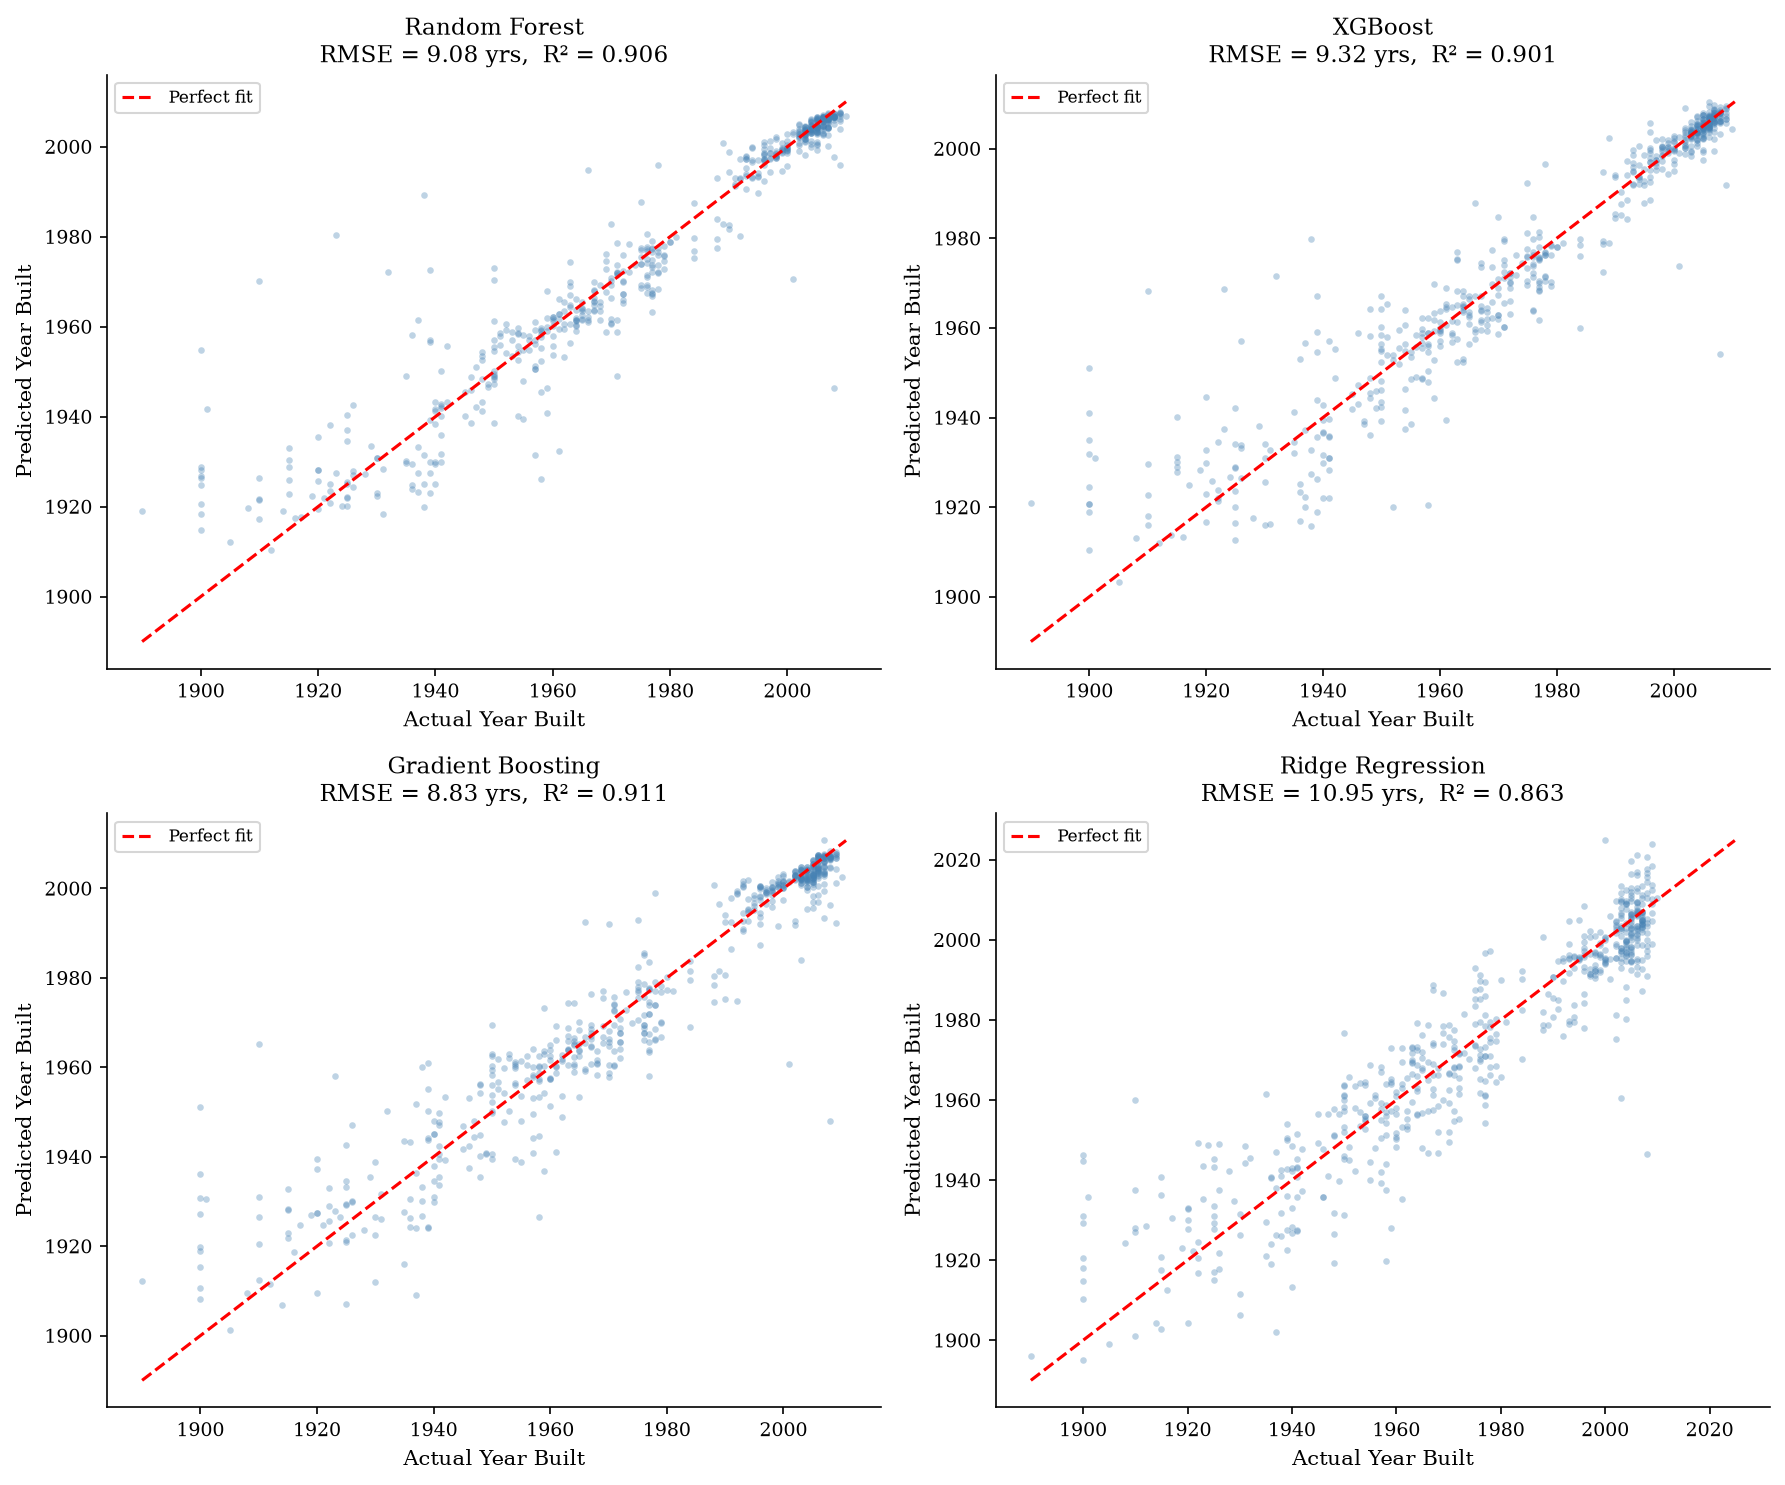
\includegraphics[width=\textwidth]{../figures/fig_predicted_vs_actual} 

}

\caption{\label{fig:pred-actual}Predicted vs actual Year Built for the four best-performing regression models. The red dashed line marks perfect prediction. RMSE and R\textsuperscript{2} are reported in each panel title.}\label{fig:fig-pred-actual}
\end{figure}

Tuning affects the four searched models unevenly (Table
\ref{tab:reg-tuned}): XGBoost improves the most, moving from third among
the default ensembles (RMSE = 9.32) to the strongest model overall after
search (RMSE = 8.40, \(R^2\) = 0.920); Gradient Boosting also improves,
though more modestly (8.83 \(\rightarrow\) 8.60); Random Forest is
essentially unchanged (9.08 \(\rightarrow\) 9.11); and SVR improves
substantially (13.09 \(\rightarrow\) 9.55) but remains well behind the
tree ensembles even after tuning. Random Forest's defaults, it seems,
were already close to optimal for this feature set; the other three had
more room for a targeted search to help.

\begin{longtable}[]{@{}lrrr@{}}
\caption{\label{tab:reg-tuned}Regression results on the held-out test
set after hyperparameter tuning (n = 586). Only the four models selected
for tuning are shown; compare against the corresponding
default-hyperparameter rows in Table
\ref{tab:reg-results}.}\tabularnewline
\toprule\noalign{}
Model & MAE (yrs) & RMSE (yrs) & R\textsuperscript{2} \\
\midrule\noalign{}
\endfirsthead
\toprule\noalign{}
Model & MAE (yrs) & RMSE (yrs) & R\textsuperscript{2} \\
\midrule\noalign{}
\endhead
\bottomrule\noalign{}
\endlastfoot
Random Forest & 4.86 & 9.11 & 0.905 \\
Gradient Boosting & 5.02 & 8.60 & 0.916 \\
XGBoost & 5.25 & 8.40 & 0.920 \\
SVR & 6.20 & 9.55 & 0.896 \\
\end{longtable}

\subsection{Classification}\label{classification}

Table \ref{tab:clf-results} covers test-set performance for all eight
classifiers. XGBoost leads on both accuracy (91.5\%) and macro F1
(0.833), with Gradient Boosting close behind (91.3\%, F1 = 0.814). The
gap between accuracy and macro F1 that shows up for most models is
really class imbalance at work: get the dominant Single-story class
right and struggle with Split-level, and accuracy still looks good even
while F1 tells a less flattering story.

\begin{longtable}[]{@{}lrrrr@{}}
\caption{\label{tab:clf-results}Classification results on the held-out
test set (n = 586). All metrics are macro-averaged across the four
typology classes.}\tabularnewline
\toprule\noalign{}
Model & Accuracy & Precision & Recall & F1 (macro) \\
\midrule\noalign{}
\endfirsthead
\toprule\noalign{}
Model & Accuracy & Precision & Recall & F1 (macro) \\
\midrule\noalign{}
\endhead
\bottomrule\noalign{}
\endlastfoot
Logistic Regression & 0.879 & 0.792 & 0.699 & 0.726 \\
Decision Tree & 0.850 & 0.736 & 0.754 & 0.744 \\
Random Forest & 0.899 & 0.897 & 0.728 & 0.763 \\
Gradient Boosting & 0.913 & 0.897 & 0.779 & 0.814 \\
XGBoost & 0.915 & 0.881 & 0.802 & 0.833 \\
SVC & 0.879 & 0.914 & 0.670 & 0.691 \\
KNN & 0.843 & 0.780 & 0.675 & 0.710 \\
Neural Network & 0.884 & 0.810 & 0.772 & 0.788 \\
\end{longtable}

Figure \ref{fig:clf-comp} (Appendix) shows this comparison visually.

Table \ref{tab:clf-cv} shows the five-fold cross-validation numbers,
scored on macro F1 and computed on the training fold only. XGBoost has
the highest mean (0.800), with Gradient Boosting (0.792) and Random
Forest (0.780) close behind, consistent with the test-set ranking, where
XGBoost also leads. Standard deviations are small for most models; KNN
is the most stable across folds (std = 0.007), while Gradient Boosting
is, somewhat surprisingly, the least stable of the ensembles (std =
0.034) despite its strong mean, a reminder that a competitive
cross-validated mean does not by itself guarantee low fold-to-fold
variance.

\begin{longtable}[]{@{}lrr@{}}
\caption{\label{tab:clf-cv}Five-fold cross-validation macro F1 for all
classification models, computed on the training fold
only.}\tabularnewline
\toprule\noalign{}
Model & CV Macro F1 mean & CV Macro F1 std \\
\midrule\noalign{}
\endfirsthead
\toprule\noalign{}
Model & CV Macro F1 mean & CV Macro F1 std \\
\midrule\noalign{}
\endhead
\bottomrule\noalign{}
\endlastfoot
Logistic Regression & 0.666 & 0.022 \\
Decision Tree & 0.742 & 0.009 \\
Random Forest & 0.780 & 0.023 \\
Gradient Boosting & 0.792 & 0.034 \\
XGBoost & 0.800 & 0.021 \\
SVC & 0.651 & 0.015 \\
KNN & 0.678 & 0.007 \\
Neural Network & 0.764 & 0.029 \\
\end{longtable}

Figure \ref{fig:clf-cv} (Appendix) shows these results visually.

Tuning affects the four classifiers unevenly (Table
\ref{tab:clf-tuned}): XGBoost improves further and remains the strongest
model overall, the Support Vector Classifier gains the most of any model
here, thanks to a wider margin parameter (\(C = 10\) against a default
of \(C = 1\)) that lets the decision boundary reach further into
minority-class territory and Gradient Boosting's tuned macro F1 dips
slightly below its untuned value, a difference small enough to chalk up
to the noise of optimising on cross-validated F1 rather than the
held-out test set directly.

\begin{longtable}[]{@{}lrrrr@{}}
\caption{\label{tab:clf-tuned}Classification results on the held-out
test set after hyperparameter tuning (n = 586). Only the four models
selected for tuning are shown; compare against the corresponding
default-hyperparameter rows in Table
\ref{tab:clf-results}.}\tabularnewline
\toprule\noalign{}
Model & Accuracy & Precision & Recall & F1 (macro) \\
\midrule\noalign{}
\endfirsthead
\toprule\noalign{}
Model & Accuracy & Precision & Recall & F1 (macro) \\
\midrule\noalign{}
\endhead
\bottomrule\noalign{}
\endlastfoot
Random Forest & 0.899 & 0.893 & 0.735 & 0.770 \\
Gradient Boosting & 0.910 & 0.884 & 0.777 & 0.811 \\
XGBoost & 0.918 & 0.884 & 0.806 & 0.837 \\
SVC & 0.896 & 0.846 & 0.765 & 0.796 \\
\end{longtable}

Figure \ref{fig:confusion} shows the confusion matrix for the default,
pre-tuning XGBoost classifier, the strongest model at that stage.
Single-story and Multi-story properties are classified well; 1.5-story
properties occasionally get mistaken for Multi-story; and Split-level
properties see the worst error rate of the four, mostly getting
predicted as Single-story or Multi-story instead.

\begin{figure}[htbp]

{\centering 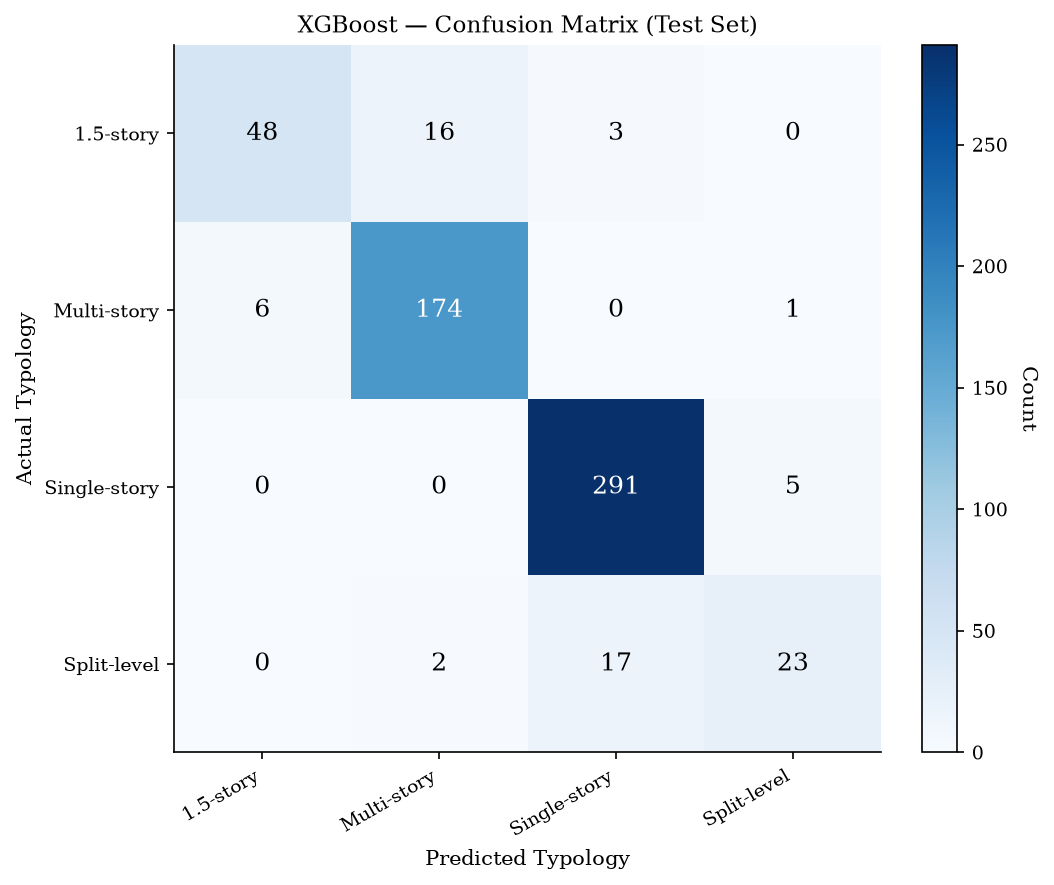
\includegraphics[width=0.7\textwidth]{../figures/fig_confusion_matrix} 

}

\caption{\label{fig:confusion}Confusion matrix for the default (pre-tuning) XGBoost classifier on the held-out test set. Rows represent actual typology classes; columns represent predicted classes.}\label{fig:fig-confusion}
\end{figure}

Each row of the matrix corresponds to one true typology (Single-story,
1.5-story, Multi-story or Split-level), and each column to the typology
the model predicted; the diagonal cells count correct predictions, while
off-diagonal cells count misclassifications between specific class
pairs. The largest diagonal counts fall on Single-story and Multi-story,
the two most frequent classes, confirming the strong recall reported for
them in Table \ref{tab:clf-results}. Off-diagonal mass concentrates on
the 1.5-story/Multi-story boundary and, more heavily, on Split-level,
which is confused with both Single-story and Multi-story more often than
it is correctly identified, reflecting the class imbalance and
structural overlap between these categories.

\section{Discussion and Conclusion}\label{discussion-and-conclusion}

\subsection{Regression Task}\label{regression-task}

Tree-based ensembles perform strongly here (Gradient Boosting
\(R^2 = 0.911\), Random Forest \(R^2 = 0.906\), XGBoost \(R^2 = 0.901\)
by default, rising to \(R^2 = 0.920\) for XGBoost after tuning), which
says a property's physical attributes really do carry a chronological
signal, and one that machine learning can recover with good accuracy.
What's more telling is how far behind the linear baselines stay
(\(R^2 \approx 0.86\)): roughly 5 percentage points of variance in
construction year simply isn't reachable by any linear combination of
predictors. That points to threshold effects rather than a smooth
relationship, which lines up with how building practice actually
evolved. Materials and design standards didn't drift continuously; they
shifted in fits and starts, driven by regulatory and technological
step-changes, and a tree's decision boundaries can represent that kind
of jump directly.

The single Decision Tree is a useful cautionary case here. Its test-set
RMSE (12.22 years, \(R^2 = 0.830\)) is clearly worse than all three tree
ensembles, despite being structurally similar to Random Forest. A single
tree has only one chance to pick the best available split at each node,
so it is more exposed to whichever predictor looks strongest in the
training data at that point, including predictors that turn out to
generalise poorly; bagging (Random Forest) and boosting (Gradient
Boosting, XGBoost) both average over many such trees and are
correspondingly more robust to this.

The default SVR falls behind the other non-linear methods (RMSE = 13.09,
\(R^2 = 0.805\)), which suggests its default radial basis function
kernel just isn't matched well to this dataset's structure. Tuning
narrows that gap substantially (RMSE drops to 9.55, Table
\ref{tab:reg-tuned}), so the shortfall looks more like a hyperparameter
problem than a fundamental mismatch between margin-based methods and
this task. Even tuned, though, the SVR stays well behind the ensembles,
a structural disadvantage on this high-dimensional, mixed-type feature
set that tuning alone doesn't fully close.

The neural network's cross-validation variance (RMSE = 14.85 \(\pm\)
1.99) sits well above both its own test-set result (10.53) and every
tree-based model's CV variance. That's a sign of fold-dependent
performance rather than genuine generalisation. With only 2,344 training
observations against 147 post-encoding features, the default
architecture probably doesn't have the capacity to exploit deep
interaction effects consistently, and the uneven temporal spread of
observations across folds doesn't make its job any easier.

\subsection{Classification Task}\label{classification-task}

The classification results show architectural typology can be recovered
from geometric measurements with reasonable accuracy. XGBoost leads both
before tuning (91.5\% accuracy, macro F1 = 0.833) and after (91.8\%, F1
= 0.837), which makes it the strongest model in either task once tuning
is accounted for. The gap between accuracy and macro F1 tells the
class-imbalance story again: the untuned SVC posts 87.9\% accuracy but a
macro F1 of only 0.691, dragged down by weak recall (0.670) on the
minority classes. Its precision (0.914) is high, though, which points to
conservative decision boundaries: the model rarely commits to a
minority-class prediction unless it's confident. Tuning fixes most of
this (macro F1 climbs to 0.796, Table \ref{tab:clf-tuned}), confirming
the untuned SVC's weakness was a hyperparameter problem rather than
something inherent to margin-based classifiers on this feature set. The
same pattern shows up in the confusion matrix (Figure
\ref{fig:confusion}): Split-level properties, only 7.2\% of the dataset,
get misclassified more often than any other class.

There's a straightforward architectural reason behind the confusion
between 1.5-story and Multi-story properties, and between Split-level
and Single-story ones. Both 1.5-story and split-level homes sit in an
awkward middle ground: a one-and-a-half story home has only a partial
upper storey, and a split-level home has partial floors set at offset
heights. The 30-feature geometric representation captures aggregate
measurements (total area, room counts, basement footprint) but not the
volumetric arrangement that would actually distinguish these forms from
a full two-story layout. No model choice fixes that; the ceiling on
accuracy is baked into the feature set itself. This lines up with the
EDA finding in Figure \ref{fig:clf-eda}: \texttt{2nd\ Flr\ SF} separates
Multi-story from Single-story and Split-level cleanly, but 1.5-story
properties sit in between with substantial overlap on both sides, which
is exactly where the confusion matrix shows the models struggling most.

One further point is worth flagging explicitly: the untuned Neural
Network's macro F1 (0.788, Table \ref{tab:clf-results}) exceeds the
tuned Random Forest's (0.770, Table \ref{tab:clf-tuned}). This is not
evidence that tuning failed in any general sense; a hyperparameter
search optimises cross-validated performance on the training fold, which
does not guarantee an improvement on every other model's held-out result
on one particular split. It is a reminder that a single train/test
comparison should not be read as a strict ranking of tuning outcomes
across different models.

\subsection{Model Interpretability}\label{model-interpretability}

The two best regression models, Random Forest and XGBoost, offer partial
interpretability through feature importance. Extracting
mean-decrease-in-impurity importance from both fitted default models
(Figure \ref{fig:feat-imp}) tells a more specific story than the
correlation ranking in Section \ref{exploratory-data-analysis} on its
own would suggest: \texttt{Bsmt\ Qual}, the ordinal basement-quality
rating, dominates both models (55\% of total importance for Random
Forest, 40\% for XGBoost), with the one-hot encoded \texttt{Foundation}
categories (\texttt{PConc}, \texttt{BrkTil}, \texttt{CBlock}) taking
over as a distant second, third and fourth for both, now that the two
excluded temporal fields (\texttt{Year\ Remod/Add\ Delta},
\texttt{Garage\ Yr\ Blt}) are out of the feature set entirely.
\texttt{Overall\ Qual} and \texttt{Gr\ Liv\ Area}, despite their visible
correlation with \texttt{Year\ Built} in the exploratory analysis, do
not appear among either model's top ten features. This is a useful
illustration of why marginal correlation and model-internal feature
importance are not interchangeable: \texttt{Bsmt\ Qual} is a categorical
quality rating that both tree ensembles can split on cleanly, and it
plausibly proxies changing basement-finishing standards across
construction eras more directly than raw floor area does; foundation
type follows a similar logic, since poured concrete (\texttt{PConc})
foundations only became the dominant choice later in the sample window,
displacing older brick/tile (\texttt{BrkTil}) and block construction.
This is a predictive association within these two specific models, not a
causal claim about what determines a house's construction year. If
understanding what's actually driving a given prediction matters,
XGBoost paired with SHAP values is the more useful option at the
instance level.

\begin{figure}[htbp]

{\centering \includegraphics[width=\textwidth]{../figures/fig_feature_importance} 

}

\caption{\label{fig:feat-imp}Mean-decrease-in-impurity feature importance for the default Random Forest and XGBoost regressors (top 10 features each). Prefixes indicate the preprocessing group each feature belongs to (ordinal, standardised, normalised, one-hot or binary encoded).}\label{fig:fig-feat-imp}
\end{figure}

The linear models, Linear Regression and Ridge, offer full
coefficient-level interpretability, but it costs roughly 2.5 RMSE years
relative to the best-performing ensemble (XGBoost, tuned). Where
interpretability is the binding constraint and approximate accuracy is
good enough, Ridge Regression makes sense. Otherwise, the performance
gap is large enough to justify going with Gradient Boosting or XGBoost
instead.

The classification versions of Gradient Boosting and XGBoost offer the
same kind of interpretability as their regression counterparts.
Extracting mean-decrease-in-impurity importance from the tuned Random
Forest and XGBoost classifiers (Figure \ref{fig:clf-feat-imp}) confirms
what the EDA in Figure \ref{fig:clf-eda} already suggested:
\texttt{2nd\ Flr\ SF} is overwhelmingly the most important predictor for
both models (31\% of total importance for Random Forest, 33\% for
XGBoost), well ahead of \texttt{Total\ Bsmt\ SF}/\texttt{Half\ Bath} for
Random Forest and \texttt{Half\ Bath}/\texttt{Low\ Qual\ Fin\ SF} for
XGBoost. This is a case where the exploratory analysis and the
model-internal importance agree, which is reassuring, but it is still a
predictive association within these fitted models rather than a claim
that second-floor area causes a particular architectural style: a
house's typology is fixed at construction, and \texttt{2nd\ Flr\ SF} is
simply the clearest observable trace of it.

\begin{figure}[htbp]

{\centering \includegraphics[width=\textwidth]{../figures/fig_clf_feature_importance} 

}

\caption{\label{fig:clf-feat-imp}Mean-decrease-in-impurity feature importance for the tuned Random Forest and XGBoost classifiers (top 10 features each).}\label{fig:fig-clf-feat-imp}
\end{figure}

The Decision Tree, despite lower accuracy, is the most transparent model
of all: a single tree can be drawn out in full, and every prediction
traced through an explicit sequence of attribute thresholds. Decision
Tree accuracy (85.0\%) sits close enough to Logistic Regression's
(87.9\%) that non-linear boundaries alone can't explain why the
ensembles do better; variance reduction through aggregation is doing at
least as much work.

\subsection{Practical Implications}\label{practical-implications}

Both tasks are motivated by the same practical situation: a property
record with physical measurements but incomplete or unreliable metadata.
Recovering construction year with an error of only a few years is
precise enough to support tasks such as flagging likely mis-recorded or
missing build dates for manual review, or providing a plausible estimate
where none is on file. Recovering architectural typology from geometry
alone is useful in a similar way, for example to sanity-check or
auto-populate a style field in a property database from structural
measurements that are already recorded elsewhere. Neither result is
precise enough to replace an authoritative source (a deed, a permit
record) where one exists; the value is in filling gaps or catching
errors in datasets where such a source is missing or unreliable.

\subsection{Limitations}\label{limitations}

Both tasks are evaluated on data from one city over a four-year window.
The chronological signal the regression model relies on reflects
construction norms specific to Ames, Iowa, and there's no guarantee it
would transfer to a different geographic or cultural setting. The
four-class typology grouping used here is also just one reasonable
choice among several; a different grouping would draw different class
boundaries and could well change which classifiers struggle and where.

Some of the geometric features kept in the classification set (garage
size, basement finish level) are themselves correlated with construction
era. That opens the possibility that the model is partly exploiting an
indirect temporal signal rather than purely spatial information. Teasing
the two apart would need a more controlled feature selection procedure,
or a residualisation approach.

\subsection{Conclusion}\label{conclusion}

Residential properties in the Ames Housing Dataset carry two forms of
latent architectural information, construction era and structural
typology, and both turn out to be recoverable with good accuracy.
XGBoost, after hyperparameter tuning, gives the strongest regression
performance (RMSE = 8.40 years, \(R^2\) = 0.920); tuned XGBoost also
gives the strongest classification performance (accuracy = 91.8\%, macro
F1 = 0.837). Tree-based ensembles, bagged (Random Forest) or boosted
(Gradient Boosting, XGBoost), consistently beat the linear,
kernel-based, and instance-based alternatives in both tasks, and
cross-validation confirms these results hold up rather than being an
artefact of one lucky train/test split.

Methodologically, three things keep coming up here that apply well
beyond this dataset: leakage-safe preprocessing pipelines are worth the
setup cost, evaluation metrics need to account for class imbalance
rather than default to accuracy and predictive power always trades off
against interpretability to some degree. The \texttt{MS\ SubClass} and
\texttt{Garage\ Yr\ Blt} cases in Section \ref{data-preprocessing} are
concrete illustrations of the first point: a variable can look like an
unremarkable numeric predictor and still carry an indirect encoding of
the target, or duplicate it under a different name, and this is only
caught by checking what a feature actually represents, not just how it
is typed or scaled. When the accuracy margin is large enough to justify
it, ensemble methods strike a good balance: strong generalisation paired
with partial explainability through feature importance, which is exactly
the combination that makes them well suited to structured prediction
tasks on housing data.

\appendix

\section*{Appendix}\label{appendix}
\addcontentsline{toc}{section}{Appendix}

The figures and table below supplement the results discussed in the main
text; the accompanying test-set and cross-validation tables report the
same information numerically.

\begin{figure}[htbp]

{\centering 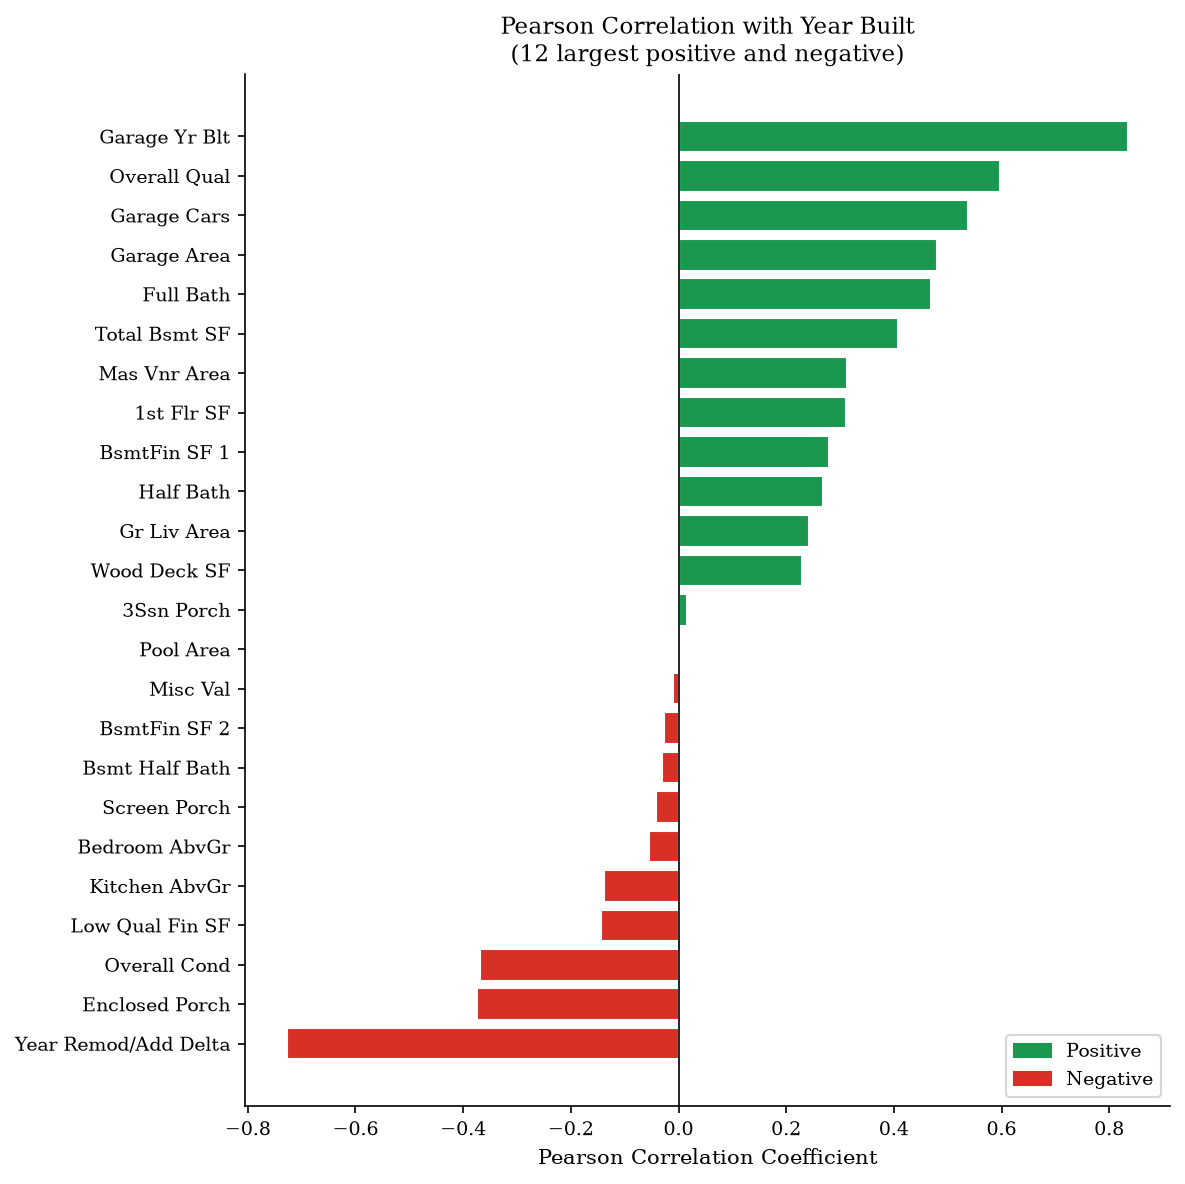
\includegraphics[width=0.85\textwidth]{../figures/fig_correlation} 

}

\caption{\label{fig:correlation}Pearson correlation between numerical predictors and Year Built. Green bars indicate positive correlations; red bars indicate negative correlations. The 12 strongest in each direction are shown.}\label{fig:fig-correlation}
\end{figure}

\begin{figure}[htbp]

{\centering 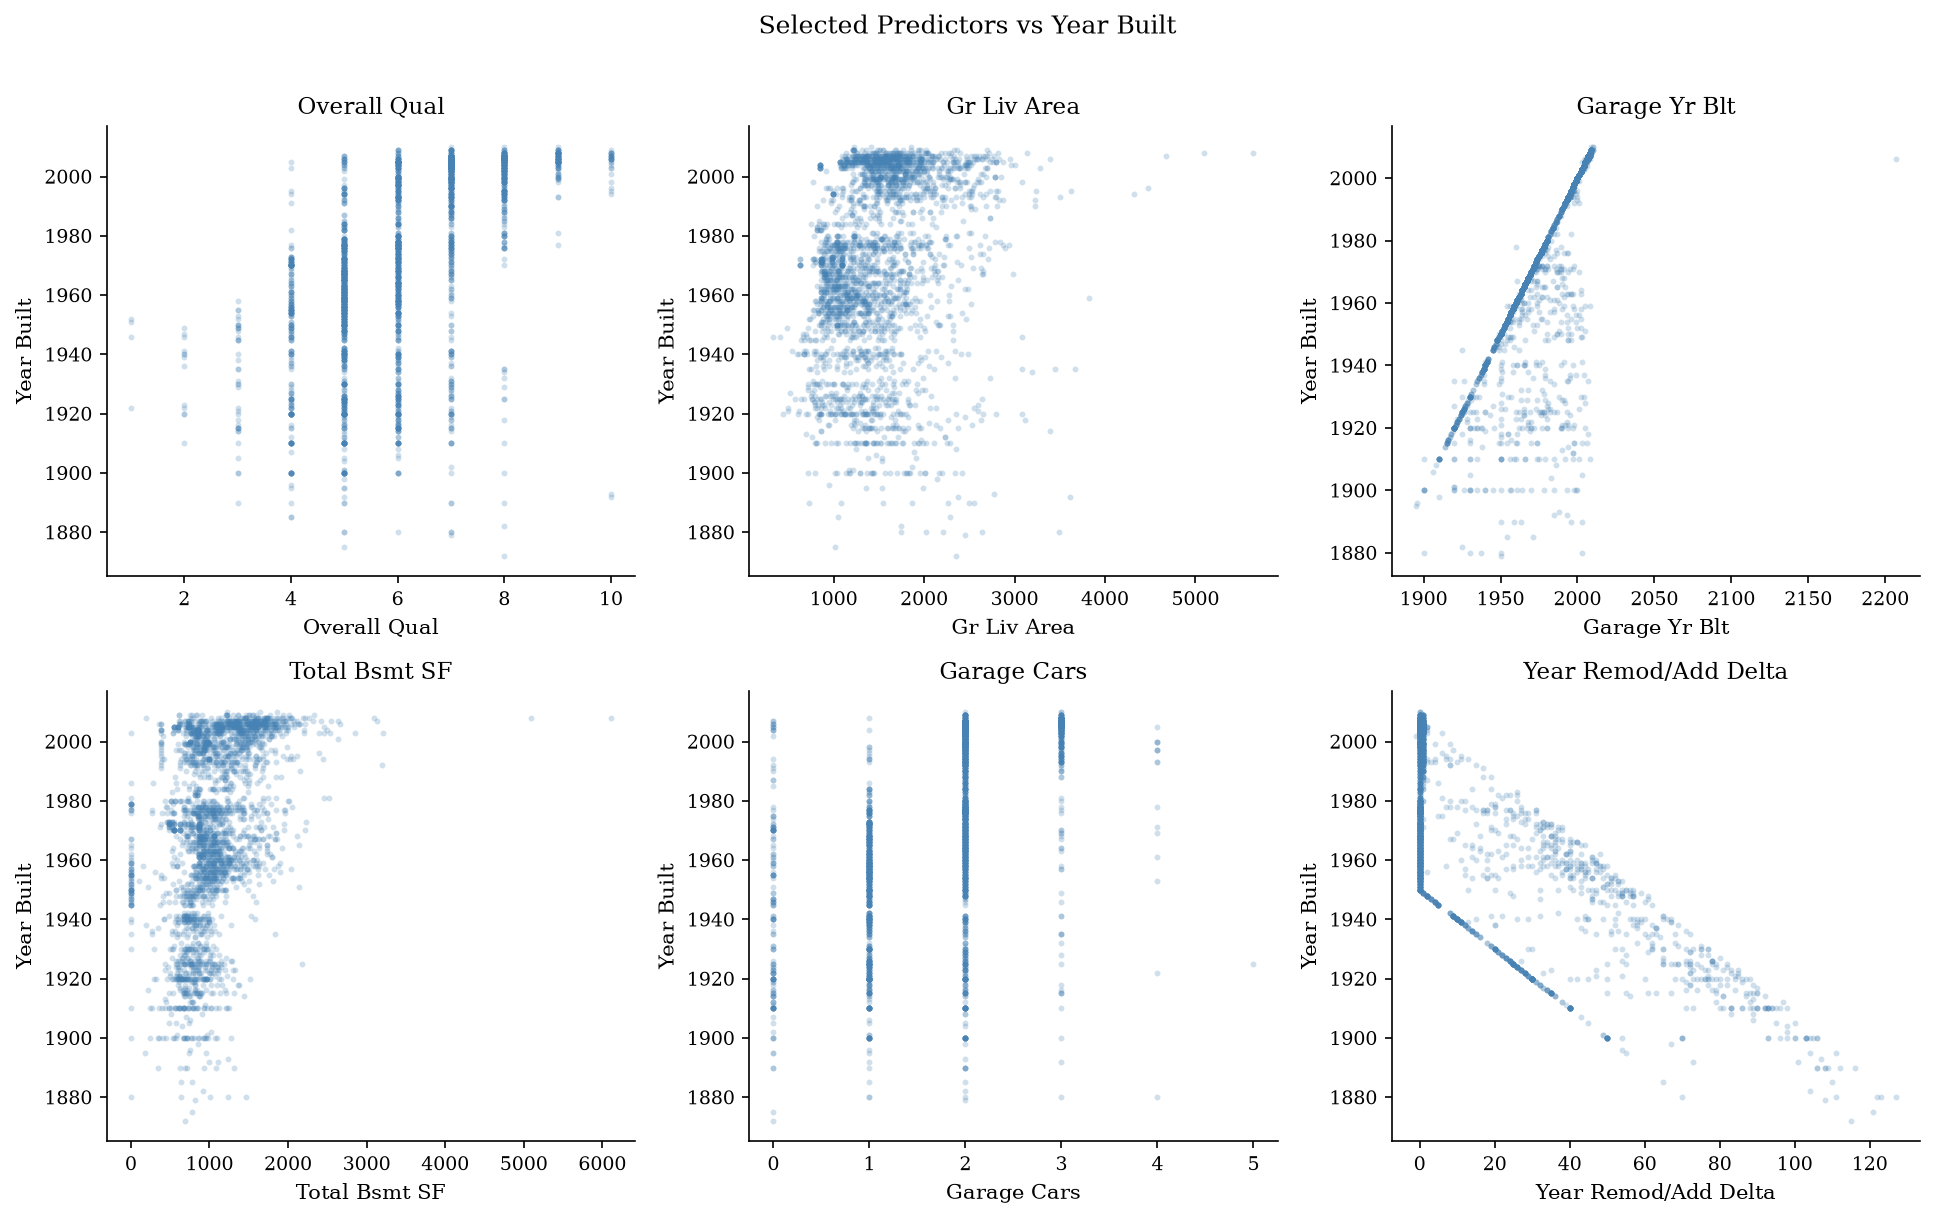
\includegraphics[width=\textwidth]{../figures/fig_scatter_predictors} 

}

\caption{\label{fig:scatter}Scatter plots of six key numerical predictors against Year Built. Each point represents one property.}\label{fig:fig-scatter}
\end{figure}

\begin{longtable}[]{@{}
  >{\raggedright\arraybackslash}p{(\linewidth - 4\tabcolsep) * \real{0.1845}}
  >{\raggedright\arraybackslash}p{(\linewidth - 4\tabcolsep) * \real{0.1786}}
  >{\raggedright\arraybackslash}p{(\linewidth - 4\tabcolsep) * \real{0.6369}}@{}}
\caption{\label{tab:hp-grid}Full hyperparameter search space for each
tuned model. Random Forest's grid differs slightly between tasks;
Gradient Boosting, XGBoost and SVR/SVC use the same grid for both
(selected values reported in Table
\ref{tab:hp-selected}).}\tabularnewline
\toprule\noalign{}
\begin{minipage}[b]{\linewidth}\raggedright
Model
\end{minipage} & \begin{minipage}[b]{\linewidth}\raggedright
Search method
\end{minipage} & \begin{minipage}[b]{\linewidth}\raggedright
Hyperparameters searched
\end{minipage} \\
\midrule\noalign{}
\endfirsthead
\toprule\noalign{}
\begin{minipage}[b]{\linewidth}\raggedright
Model
\end{minipage} & \begin{minipage}[b]{\linewidth}\raggedright
Search method
\end{minipage} & \begin{minipage}[b]{\linewidth}\raggedright
Hyperparameters searched
\end{minipage} \\
\midrule\noalign{}
\endhead
\bottomrule\noalign{}
\endlastfoot
Random Forest (regression) & RandomizedSearchCV (10 iter.) &
n\_estimators \{50,100,200\}; max\_depth \{None,10,20,30\};
min\_samples\_split \{2,5,10\}; min\_samples\_leaf \{1,2,4\} \\
Random Forest (classification) & RandomizedSearchCV (10 iter.) &
n\_estimators \{50,100,200\}; max\_depth \{None,10,20\};
min\_samples\_split \{2,5,10\} \\
Gradient Boosting & GridSearchCV & n\_estimators \{50,100,200\};
learning\_rate \{0.01,0.1,0.2\}; max\_depth \{3,5,7\} \\
XGBoost & RandomizedSearchCV (10 iter.) & n\_estimators \{50,100,200\};
learning\_rate \textasciitilde{} Uniform(0.01, 0.31); max\_depth
\{3,5,7\} \\
SVR / SVC & GridSearchCV & kernel \{linear, rbf\}; C \{0.1,1,10\}; gamma
\{scale, auto\} \\
\end{longtable}

\begin{figure}[htbp]

{\centering 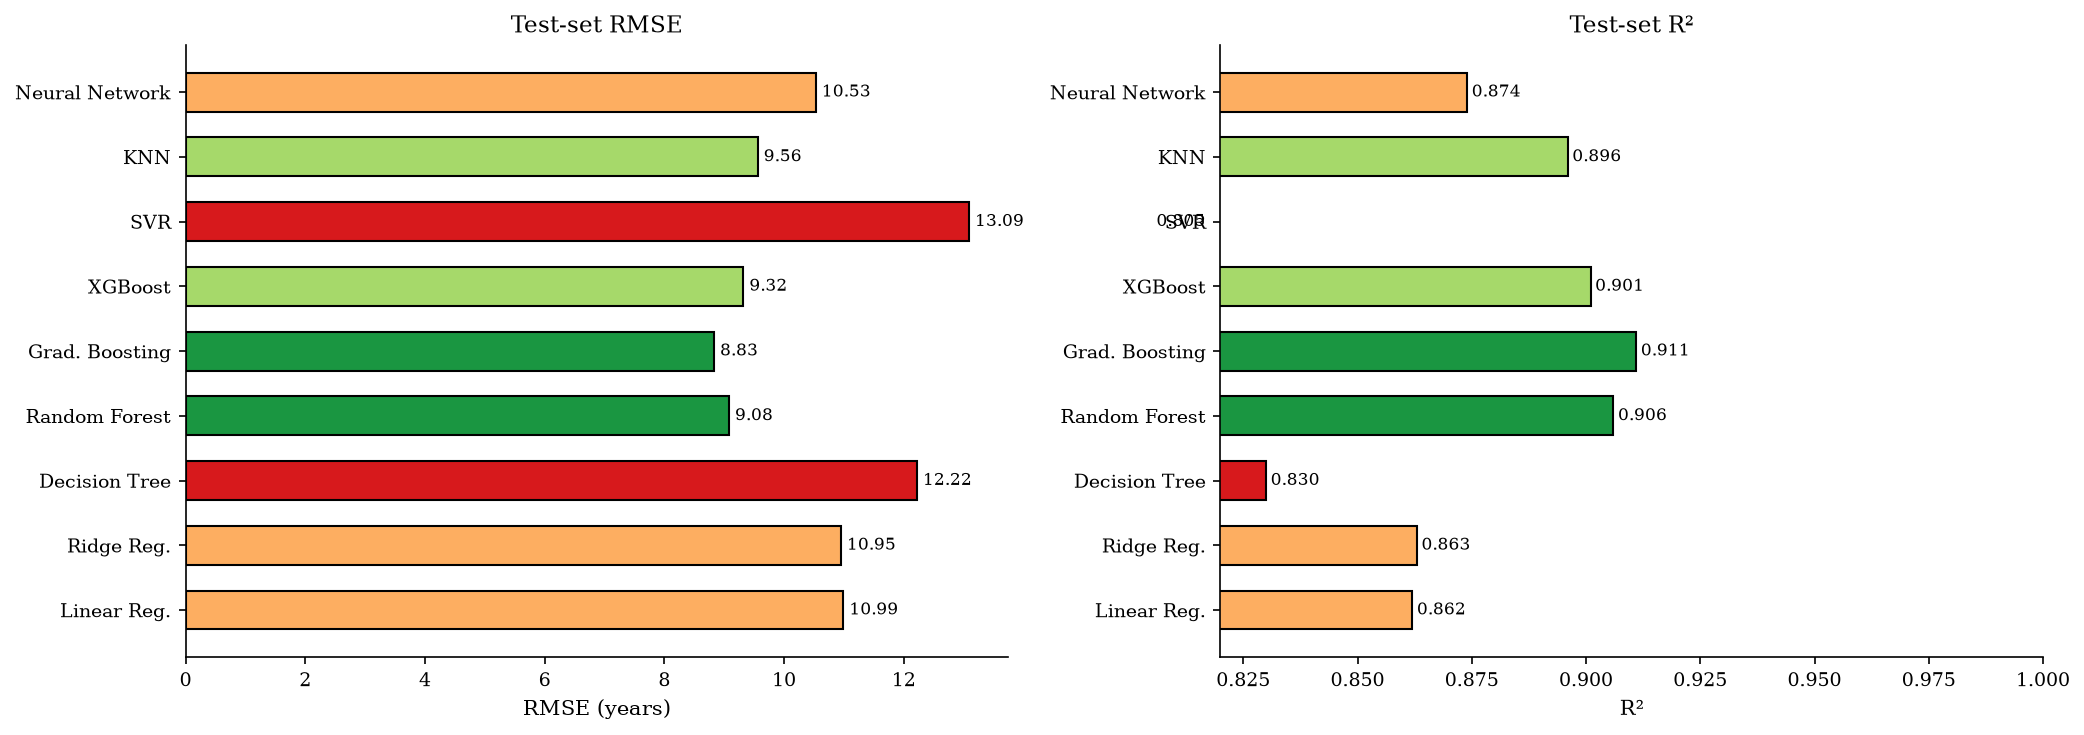
\includegraphics[width=\textwidth]{../figures/fig_reg_comparison} 

}

\caption{\label{fig:reg-comp}Comparison of all nine regression models by test-set RMSE (left) and R\textsuperscript{2} (right). Colour indicates rank: green = top 2, light green = ranks 3--4, orange = ranks 5--7, red = bottom 2.}\label{fig:fig-reg-comp}
\end{figure}

\begin{figure}[htbp]

{\centering 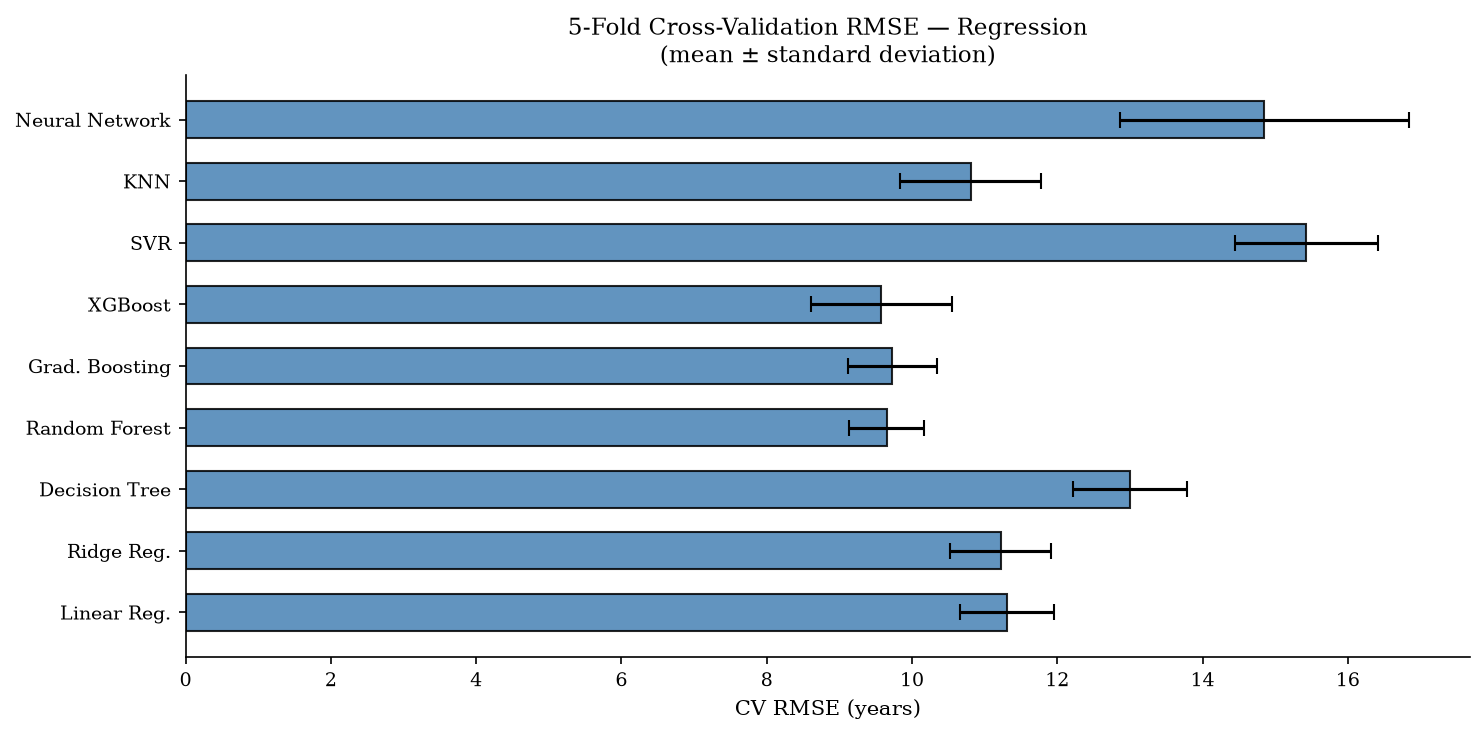
\includegraphics[width=\textwidth]{../figures/fig_reg_cv} 

}

\caption{\label{fig:reg-cv}Five-fold cross-validation RMSE for all regression models (mean $\pm$ standard deviation).}\label{fig:fig-reg-cv}
\end{figure}

\begin{figure}[htbp]

{\centering 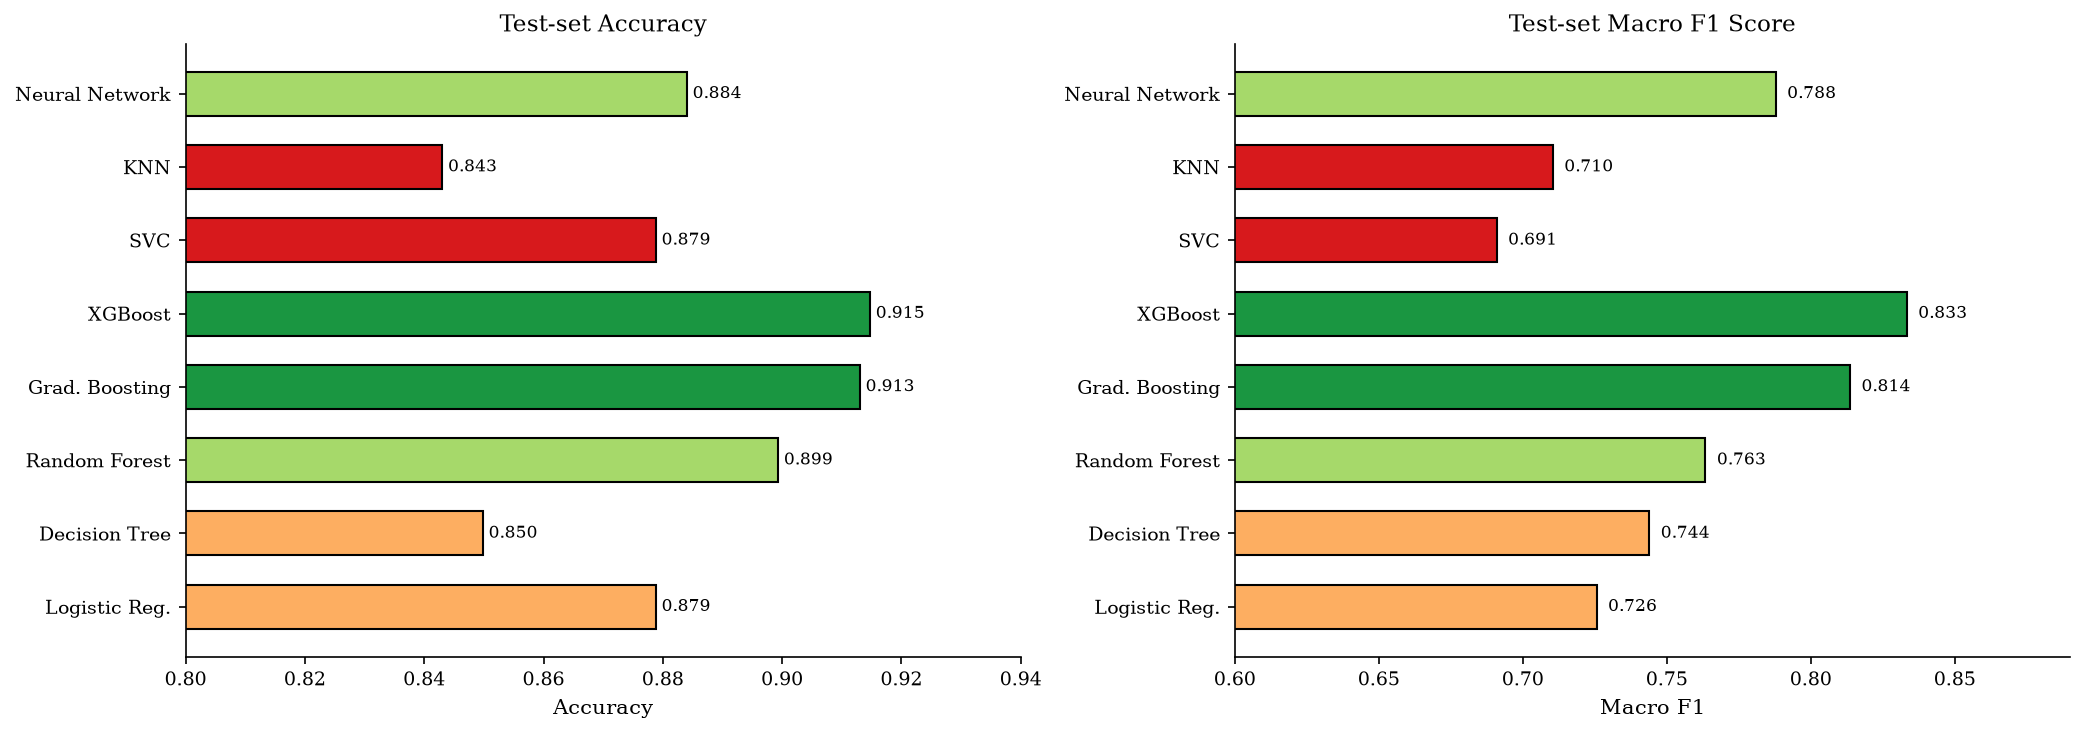
\includegraphics[width=\textwidth]{../figures/fig_clf_comparison} 

}

\caption{\label{fig:clf-comp}Comparison of all eight classification models by test-set accuracy (left) and macro F1 score (right).}\label{fig:fig-clf-comp}
\end{figure}

\begin{figure}[htbp]

{\centering 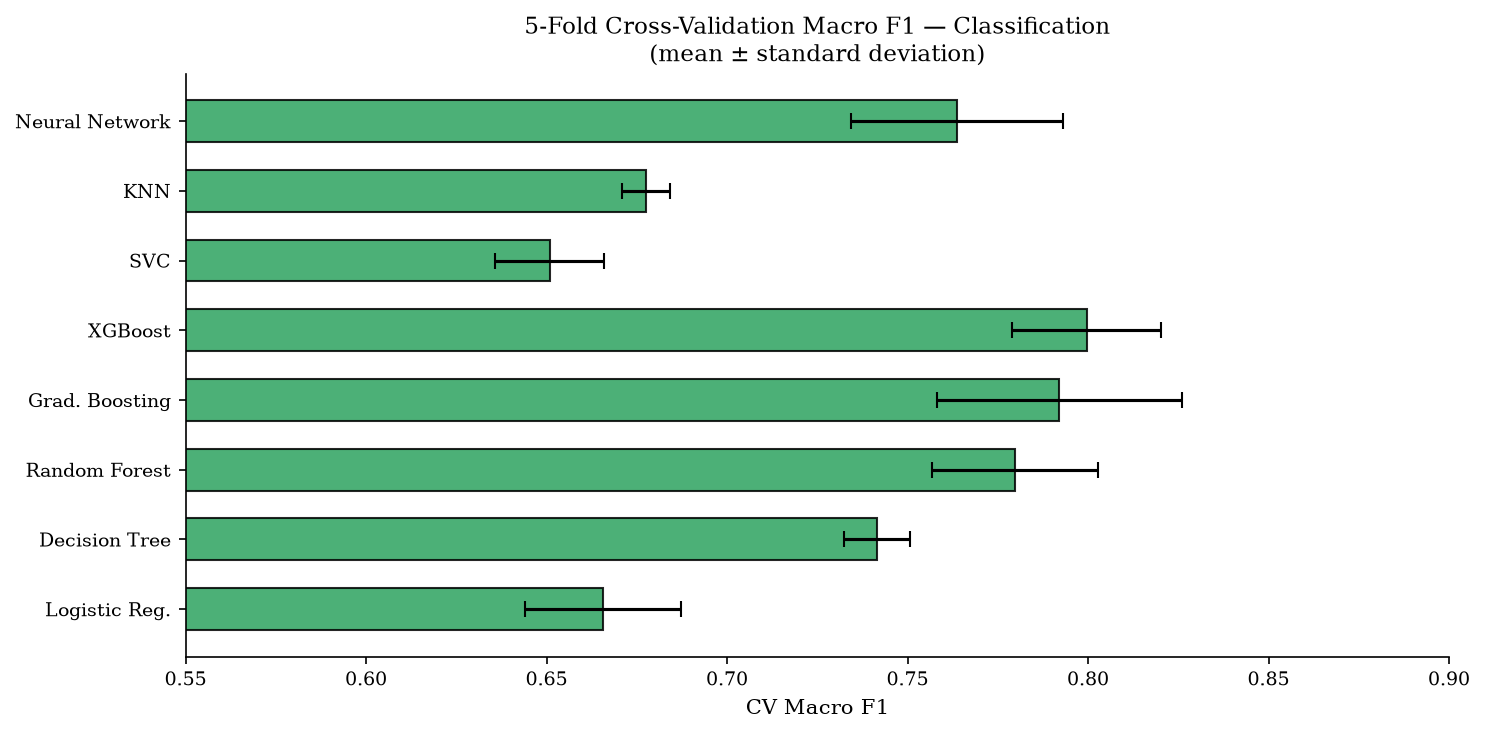
\includegraphics[width=\textwidth]{../figures/fig_clf_cv} 

}

\caption{\label{fig:clf-cv}Five-fold cross-validation macro F1 for all classification models (mean $\pm$ standard deviation).}\label{fig:fig-clf-cv}
\end{figure}

\begingroup
\raggedright
\printbibliography[title=References]
\endgroup

\end{document}
